\documentclass[12pt,a4paper]{report}

% ===== Fonts & encoding =====
\usepackage[T1]{fontenc}
\usepackage{newtxtext} % Times-like text
\usepackage{newtxmath} % Times-like math

% ===== Layout & formatting =====
\usepackage{geometry}
\geometry{left=1.25in,right=1in,top=1in,bottom=1in}
\usepackage{setspace}
\setstretch{1.2}

\usepackage{graphicx}
\usepackage{xcolor}
\usepackage[most]{tcolorbox}
\usepackage{array}
\usepackage{enumitem}
\usepackage{longtable}
\usepackage{titlesec}
\usepackage{fancyhdr}
\usepackage[hidelinks]{hyperref}
\usepackage{cite} % numeric citations like [1]

% ===== Springer-like floats & math =====
\let\Bbbk\relax
\usepackage{amsmath,amssymb}
\usepackage{booktabs}
\usepackage{algorithm}
\usepackage{algpseudocode}

% ===== Colors (tuned to the sample) =====
\definecolor{christBlue}{HTML}{1F4E79}
\definecolor{christGold}{HTML}{8A6A1B}
\definecolor{christGreen}{HTML}{2E7D32}
\definecolor{christGray}{HTML}{E9EDF5}

% ===== Header block used on the formatted front pages =====
\newcommand{\ChristHeader}{%
  \begin{center}
    
\includegraphics[width=9cm,height=2.7cm]{images/cunamelogo.png}\\[-2pt]
  \end{center}
}

% ===== Box styles for front-matter design pages =====
\tcbset{
  christbox/.style={
    enhanced,
    colback=white,
    boxrule=1.3pt,
    arc=2mm,
    left=6mm,right=6mm,top=3mm,bottom=3mm,
  },
  christbluebox/.style={christbox,colframe=christBlue},
  christgoldbox/.style={christbox,colframe=christGold},
  christgreenbox/.style={christbox,colframe=christGreen,colback=christGreen!5},
  christgraybox/.style={christbox,colframe=black!50,colback=christGray,fontupper=\large},
}

% ===== Page style =====
\pagestyle{fancy}
\fancyhf{}
\fancyfoot[R]{\thepage}
\renewcommand{\headrulewidth}{0pt}

% ===== Common data (Exact Official Labmentix Details) =====
\newcommand{\StudentName}{Shreya Sunil Morajkar}
\newcommand{\StudentRegNo}{2362035}
\newcommand{\DepartmentName}{Department of Computer Science and Engineering}
\newcommand{\SchoolName}{School of Engineering and Technology}
\newcommand{\UniversityName}{CHRIST (Deemed to be University)}
\newcommand{\CampusAddress}{Kumbalagudu, Bengaluru - 560 074}
\newcommand{\DegreeName}{Bachelor of Technology}
\newcommand{\SpecializationName}{Computer Science and Engineering}
\newcommand{\GuideName}{Faculty Guide Name}
\newcommand{\HODName}{Head of the Department}
\newcommand{\IndustryGuideName}{Swaraj Phatangade (Founder \& CEO)}
\newcommand{\CompanyName}{Labmentix Pvt. Ltd.}
\newcommand{\CompanyAddress}{Bengaluru, Karnataka 560029}
\newcommand{\InternshipTitle}{SmartERP: Keyboard-Driven Billing, Inventory and Double-Entry Accounting Management System}
\newcommand{\CourseCodeName}{CSE431 -- Summer Internship}
\newcommand{\InternshipStartDate}{01st April 2026}
\newcommand{\InternshipEndDate}{01st August 2026}
\newcommand{\InternshipVivaDate}{September 2026}
\newcommand{\DeclarationDate}{08th August 2026}
\newcommand{\InternshipDurationDays}{120 (4 Months)}
\newcommand{\CoverMonthYear}{September -- 2026}
\newcommand{\AcademicYearText}{2026--27}

% ===== Cover/header/footer block to match the provided sample =====
\newcommand{\ChristBlueHeader}{%
  \colorbox{christBlue}{%
    \parbox{\dimexpr\textwidth-2\fboxsep\relax}{%
      \color{white}\sffamily
      \begin{minipage}[c]{0.72\textwidth}
        \footnotesize\bfseries \MakeUppercase{\DepartmentName}\\[-1pt]
        \scriptsize\mdseries \SchoolName
      \end{minipage}%
      \hfill
      \begin{minipage}[c]{0.24\textwidth}
        \raggedleft
        
\includegraphics[height=10mm]{images/cunamelogo_blue.png}
      \end{minipage}%
    }%
  }%
}

\fancypagestyle{christcover}{%
  \fancyhf{}
  \renewcommand{\headrulewidth}{0pt}
  \fancyhead[C]{\ChristBlueHeader}
  \fancyfoot[C]{\sffamily\footnotesize Academic Year: \AcademicYearText}
}

% ===== Chapter heading formatting =====
\titleformat{\chapter}[display]
  {\bfseries\centering}
  {\MakeUppercase{\chaptername\ \thechapter}}
  {6pt}
  {\MakeUppercase}
\titlespacing*{\chapter}{0pt}{-10pt}{18pt}

% Rename bibliography heading
\renewcommand{\bibname}{References}

\begin{document}

% ===== Front matter =====
\begin{titlepage}
% No header/footer on the cover page
\thispagestyle{empty}
\ChristHeader
\vspace*{1.5cm}
\begin{center}
  {\large \bfseries An Internship Report on}\\[1.2cm]
  {\Large \bfseries \InternshipTitle}\\[1 cm]

  {\normalsize Submitted partial fulfillment of the requirements for the degree of}\\[1.0 cm]
  {\Large \bfseries \MakeUppercase{\DegreeName}}\\[3pt]
  {\normalsize in}\\[3pt]
  {\normalsize \bfseries \SpecializationName}\\[1.0cm]

  {\normalsize By}\\[6pt]
  {\normalsize \bfseries \StudentName \hspace{0.3cm}(\StudentRegNo)}\\[2.0cm]

  {\normalsize Under the Guidance of}\\[6pt]
  {\normalsize \bfseries \GuideName}\\[2.0cm]

  {\normalsize \bfseries \DepartmentName}\\[2pt]
  {\normalsize \bfseries \SchoolName,}\\[2pt]
  {\normalsize \bfseries \UniversityName,\\ \CampusAddress}\\[10pt]

  {\normalsize \bfseries \CoverMonthYear}
\end{center}
\end{titlepage}


\pagenumbering{roman}
\setcounter{page}{1}

\clearpage
\thispagestyle{empty}
\ChristHeader

\vspace{0.5cm}

\begin{center}
  {\color{christBlue}\bfseries\LARGE Vision\par}
\end{center}
\vspace{0.1cm}
\begin{tcolorbox}[christbluebox]
\centering\itshape ``Excellence and Service''
\end{tcolorbox}

\vspace{0.5cm}

\begin{center}
  {\color{christBlue}\bfseries\LARGE Mission\par}
\end{center}
\vspace{0.1cm}
\begin{tcolorbox}[christgoldbox]
\itshape CHRIST (Deemed to be University) is a nurturing ground for an individual’s holistic development to make effective contribution to the society in a dynamic environment.
\end{tcolorbox}

\vspace{0.5cm}

\begin{center}
  {\color{christBlue}\bfseries\LARGE Core Values\par}
\end{center}
\vspace{0.1cm}
\begin{tcolorbox}[christgreenbox]
\centering\itshape
Faith in God\\
Moral Uprightness\\
Love of Fellow Beings\\
Social Responsibility\\
Pursuit of Excellence
\end{tcolorbox}

\clearpage
\thispagestyle{empty}
\ChristHeader

\vspace{0.3cm}

\begin{center}
  {\color{christBlue}\bfseries\LARGE Department Vision\par}
\end{center}
%\vspace{0.1cm}
\begin{tcolorbox}[christbluebox]
\centering\itshape ``To fortify Ethical Computational Excellence''
\end{tcolorbox}

\vspace{0.3cm}

\begin{center}
  {\color{christBlue}\bfseries\LARGE Department Mission\par}
\end{center}
%\vspace{0.1cm}
\begin{tcolorbox}[christgoldbox]
\begin{description}
  \item[\textbf{M1:}] \textit{Imparts core and contemporary knowledge in the areas of Computation and Information Technology.}
  \item[\textbf{M2:}] \textit{Promotes the culture of research and facilitates higher studies.}
  \item[\textbf{M3:}] \textit{Acquaints the students with the latest  industrial practices, team building and entrepreneurship.}
 \item[\textbf{M4:}] \textit{Sensitizes the students to serve for environmental, social & ethical needs of society through lifelong learning.}
  %\item[\textbf{M5:}] \textit{Department Mission5.}
\end{description}
\end{tcolorbox}

\vspace{0.3cm}

\begin{center}
  {\color{christBlue}\bfseries\LARGE Program Educational Objectives (PEOs)\par}
\end{center}
%\vspace{0.1cm}
\begin{tcolorbox}[christgreenbox]
\begin{description}
  \item[\textbf{PEO1:}] \textit{Professional Acumen: Understand, analyze and design solutions with professional competency for the real-world problems.}
  \item[\textbf{PEO2:}] \textit{Critical Analysis: Develop software/embedded solutions for the requirements, based on critical analysis and research.}
  \item[\textbf{PEO3:}] \textit{Team work: Function effectively in a team and as an individual in a multidisciplinary/multicultural environment}
  \item[\textbf{PEO4:}] \textit{Life Long Learning: Accomplish holistic development comprehending professional responsibilities.}
  %\item[\textbf{PEO5:}] \textit{PEO5}
\end{description}
\end{tcolorbox}

\clearpage
\thispagestyle{empty}

\vspace{1.0cm}

\begin{center}
\begin{tcolorbox}[
  enhanced,
  colback=christBlue!75!black,
  colframe=christBlue!75!black,
  boxrule=0pt,
  arc=2mm,
  width=0.82\textwidth,
  left=3mm,right=3mm,top=2mm,bottom=1mm,
]
\centering\color{white}\bfseries\Large Program Outcomes (POs)
\end{tcolorbox}
\end{center}

%\vspace{0.6cm}

\begin{tcolorbox}[
  christgraybox,
  width = 1.0 \textwidth,
  arc=1mm,
  boxrule=1.3pt,
  left=5mm,right=5mm,top=1mm,bottom=1mm]
\small
\begin{description}[leftmargin=0pt,labelsep=0.6em,itemsep=0.35em,parsep=0pt]
  \item[\textbf{PO1: Engineering Knowledge}] \textit{Apply knowledge of mathematics, natural science, computing, engineering fundamentals and an engineering specialization to develop the solution of complex engineering problems.}
  \item[\textbf{PO2: Problem Analysis}] \textit{Identify, formulate, review research literature and analyze complex engineering problems reaching substantiated conclusions with consideration for sustainable development.}
  \item[\textbf{PO3: Design/Development of Solutions}] \textit{Design creative solutions for complex engineering problems and design/develop systems/components/processes to meet identified needs with consideration for the public health and safety, whole-life cost, net zero carbon, culture, society and environment as required.}
  \item[\textbf{PO4: Conduct Investigations of Complex Problems}] \textit{Conduct investigations of complex engineering problems using research-based knowledge including design of experiments, modelling, analysis \& interpretation of data to provide valid conclusions.}
  \item[\textbf{PO5: Engineering Tool Usage}] \textit{Create, select and apply appropriate techniques, resources and modern engineering \& IT tools, including prediction and modelling recognizing their limitations to solve complex engineering problems.}
  \item[\textbf{PO6: The Engineer and The World}] \textit{Analyze and evaluate societal and environmental aspects while solving complex engineering problems for its impact on sustainability with reference to economy, health, safety, legal framework, culture and environment.}
  \item[\textbf{PO7: Ethics}] \textit{Apply ethical principles and commit to professional ethics, human values, diversity and inclusion; adhere to national \& international laws.}
  \item[\textbf{PO8: Individual and Collaborative Team work}] \textit{Function effectively as an individual, and as a member or leader in diverse/multi-disciplinary teams.}
  \item[\textbf{PO9: Communication}] \textit{Communicate effectively and inclusively within the engineering community and society at large, such as being able to comprehend and write effective reports and design documentation, make effective presentations considering cultural, language, and learning differences.}
  \item[\textbf{PO10: Project Management and Finance}] \textit{Apply knowledge and understanding of engineering management principles and economic decision-making and apply these to one’s own work, as a member and leader in a team, and to manage projects and in multidisciplinary environments.}
  \item[\textbf{PO11: Life-Long Learning}] \textit{Recognize the need for, and have the preparation and ability for (i) independent and life-long learning (ii) adaptability to new and emerging technologies and (iii) critical thinking in the broadest context of technological change.}
\end{description}
\end{tcolorbox}

\clearpage
\thispagestyle{empty}

\vspace{1.0cm}

\begin{center}
\begin{tcolorbox}[
  enhanced,
  colback=christBlue!75!black,
  colframe=christBlue!75!black,
  boxrule=0pt,
  arc=2mm,
  width=0.92\textwidth,
  left=3mm,right=3mm,top=2mm,bottom=2mm,
]
\centering\color{white}\bfseries\Large Program Specific Outcomes (PSOs)
\end{tcolorbox}
\end{center}

%\vspace{0.6cm}

\begin{tcolorbox}[christgraybox]
\begin{description}
  \item[\textbf{PSO1:}]\textit{PSO1.}
  \item[\textbf{PSO2:}] \textit{PSO2}
  \item[\textbf{PSO3:}] \textit{PSO3}
  %\item[\textbf{PSO4:}] PSO4
  %\item[\textbf{PSO5:}] PSO5
\end{description}
\end{tcolorbox}

% Certificate page (formatted to match the provided sample)
\clearpage

\ChristHeader

% Line spacing (certificate page only)
\begingroup
\setstretch{1.5}

\vspace{8mm}
\begin{center}
  {\Large \bfseries \SchoolName}\\[2mm]
  {\normalsize \DepartmentName}\\[10mm]
  {\Large \bfseries CERTIFICATE}
\end{center}

\vspace{6mm}
\noindent
This is to certify that \textbf{\underline{\StudentName\ (\StudentRegNo)}} has successfully completed his/her internship work entitled ``\textbf{\InternshipTitle}'' at \textbf{\CompanyName, \CompanyAddress}, from \textbf{\InternshipStartDate{}} to \textbf{\InternshipEndDate{}} for a duration of \textbf{\InternshipDurationDays} days and submitted on \InternshipVivaDate{} in partial fulfillment for the award of \textbf{\DegreeName{}} in \textbf{\SpecializationName{}} during the academic year \textbf{\AcademicYearText}.

\vspace{30mm}
\noindent
\begin{tabular*}{\textwidth}{@{\extracolsep{\fill}}cc@{}}
  \textbf{GUIDE} & \textbf{HEAD OF THE DEPARTMENT} \\
  \GuideName & \HODName \\
  (Signature with Date) & (Signature with Seal) \\
\end{tabular*}

\endgroup

\vspace{30mm}
\noindent
\begin{tabular*}{\textwidth}{@{\extracolsep{\fill}}cc@{}}
  \textbf{EXAMINER 1} & \textbf{Examiner 2} \\
  (Name \& Signature with Date) & (Name \& Signature with Date) \\
\end{tabular*}

\chapter*{\textbf{\textit{Acknowledgement}}}

% Increase spacing between paragraphs on this page
\begingroup
\setlength{\parskip}{1cm}
\setlength{\parindent}{0pt}

We would like to thank Dr Rev Fr Joseph C. C., Vice Chancellor, CHRIST (Deemed
to be University), Dr Rev Fr Viju P. D., Pro Vice Chancellor, Dr Fr Jiby Jose,
Director, School of Engineering and Technology, Fr Shijin P. J., Assistant Director,
School of Engineering and Technology, CHRIST (Deemed to be University), Dr
Raghunandan Kumar R., Dean, and Dr Mary Anitha E. A., Associate Dean, for their
kind patronage.

We would also like to express sincere gratitude and appreciation to \textbf{\HODName},
Head of the Department, \textbf{\DepartmentName} for giving me this opportunity to take up this
project.

We also extremely grateful to my guide, \textbf{\GuideName}, who has supported and helped
to carry out the project. His constant monitoring and encouragement helped me keep
up to the project schedule.

We also extremely grateful to my co-guide, \textbf{\IndustryGuideName}, who has supported
and helped to carry out the project. His constant monitoring and encouragement helped
me keep up to the project schedule.

If outside the college-mention the organisation and the concerned people, like head of the
organisation, guide and any other person you want to thank. All faculty and non-
teaching staff. You may acknowledge your parents or any who supported you.

\endgroup

\chapter*{\textbf{\textit{Declaration}}}

% Increase spacing between paragraphs on this page
\begingroup
\setlength{\parskip}{0.7cm}
\setlength{\parindent}{0pt}

I hereby declare that the project titled \textbf{``\InternshipTitle''} is a record of the original internship work undertaken as part of the course \textbf{\CourseCodeName}, in partial fulfillment of the requirements for the award of the degree of \textbf{\DegreeName} in \textbf{\SpecializationName}.

I completed this internship under the supervision of \textbf{\GuideName} and \textbf{\IndustryGuideName}, at \textbf{\CompanyName, \CompanyAddress}, during the period from \textbf{\InternshipStartDate} to \textbf{\InternshipEndDate}.

I further declare that this internship report has not been submitted, either in whole or in part, for the award of any degree, diploma, associateship, fellowship, or any other academic qualification at any other institution. Furthermore, this report has not been submitted for publication or presentation elsewhere.

I affirm that this internship work has been carried out in accordance with the Code of Research Conduct prescribed by the University.


\vspace{1.0cm}
\textbf{Place:} \CampusAddress \\
\textbf{Date:} \DeclarationDate \\[1.2cm]
\textbf{Signature:} \StudentName\ (\StudentRegNo)

\endgroup

\chapter*{\textbf{\textit{Abstract}}}

\begingroup
\setlength{\parskip}{0.6cm}
\setlength{\parindent}{0pt}

In modern commercial accounting, speed, accuracy, and regulatory compliance are essential for high-throughput business operations. While legacy desktop ERP solutions such as Tally provide high-speed keyboard data entry, they lack cloud accessibility, multi-tenant collaboration, and modern API extensibility. Conversely, conventional web-based ERP systems often introduce UI latency and force heavy mouse interactions that hinder accountant productivity.

This internship report details the design, architecture, and implementation of \textbf{SmartERP}---a full-stack, cloud-native billing, inventory, and double-entry accounting management platform inspired by the keyboard-driven workflow of Tally ERP. Built using Next.js 16 (React 19), Express.js (Node.js), Prisma ORM, and SQLite/PostgreSQL, the application implements atomic double-entry transaction processing, multi-level inventory tracking, state-aware Indian GST computation (CGST, SGST, IGST), and real-time financial reporting including Trial Balance, Profit \& Loss, and Balance Sheet statements.

Key innovations include an event-driven keyboard shortcuts engine ($F1$--$F9$, underlined hotkeys, $ESC$ navigation stack), a context-preserving floating calculator ($F4$), spotlight command palette search ($Ctrl+K$), and automated server-side generation of GST-compliant PDF tax invoices and Excel ledger workbooks. The application's mathematical accuracy and data consistency have been thoroughly validated using an automated end-to-end integration test suite.

\textbf{Keywords:} Cloud ERP, Double-Entry Bookkeeping, Keyboard-First UI, Next.js, Express.js, Prisma ORM, GST Tax Engine, Real-Time Accounting Reports.

\endgroup


\tableofcontents
\listoffigures
\listoftables

% ===== Main matter =====
\cleardoublepage
\pagenumbering{arabic}
\setcounter{page}{1}

\chapter{Introduction}

\section{Background and Motivation}
In the modern enterprise landscape, business transactions, inventory management, and financial accounting form the backbone of commercial sustainability. For decades, computerized accounting has relied heavily on specialized desktop software such as Tally ERP. While desktop applications offer unmatched typing throughput via keyboard hotkeys, they pose significant limitations: single-machine data silos, lack of real-time remote collaboration, manual backup overhead, and absence of modern web API integrations.

Conversely, modern Software-as-a-Service (SaaS) cloud accounting platforms often introduce significant operational friction. The reliance on deep mouse menus, multi-step dropdown dialogs, and web page reloads disrupts the muscle memory of high-volume data-entry operators. 

\textbf{SmartERP} was conceived to solve this dichotomy by marrying the ergonomic, keyboard-centric data-entry paradigm of Tally with the scalability, accessibility, and real-time synchronization of modern cloud web architecture.

\section{Project Objectives}
The primary objectives of the SmartERP internship project are as follows:
\begin{itemize}
    \item \textbf{Keyboard-First Web Architecture}: Implement a comprehensive keyboard navigation subsystem supporting single-key hotkeys, function keys ($F1$--$F9$), spotlight command search ($Ctrl+K$), and contextual floating utilities ($F4$ calculator) with zero mouse dependency.
    \item \textbf{Atomic Double-Entry Engine}: Build a robust double-entry accounting engine ensuring every transaction atomically balances corresponding debit and credit ledger allocations with zero arithmetic discrepancy.
    \item \textbf{Integrated Multi-Level Inventory}: Maintain real-time stock balances linked directly to inward (Purchase) and outward (Sales) voucher transactions with automatic valuation updates.
    \item \textbf{State-Aware GST Compliance Engine}: Dynamically determine applicable Goods and Services Tax components (CGST + SGST for intra-state transactions, IGST for inter-state transactions) based on company and counterparty jurisdictions.
    \item \textbf{Instant Financial Reporting}: Provide real-time computation and rendering of Trial Balance, Profit \& Loss Account, Balance Sheet, and Stock Summary statements.
    \item \textbf{Automated Document Generation}: Implement server-side vector PDF generation for tax invoices and structured Excel workbook exports for audit compliance.
\end{itemize}

\section{Organization Profile --- Labmentix}
\textbf{Labmentix} is a technology innovation and software development organization focused on building scalable cloud enterprise solutions, data engineering systems, and empowering engineering students with hands-on industrial full-stack experience. 

During the internship tenure, the intern was embedded within the Core Product Development team at Labmentix, collaborating on full-stack architecture design, database schema modeling, front-end optimization, and test-driven development under the guidance of technical mentors.

\section{Scope of the Internship Work}
The internship encompassed end-to-end software development lifecycle (SDLC) responsibilities:
\begin{enumerate}
    \item \textbf{Requirements Gathering \& Design}: Formulating accounting logic, Tally-inspired UX wireframes, and relational database schema.
    \item \textbf{Backend Development}: Engineering Express.js REST API routes, Prisma ORM schema models, and transactional double-entry logic.
    \item \textbf{Frontend Development}: Developing the Next.js 16 App Router interface, keyboard event listener hooks, and reactive Tailwind UI components.
    \item \textbf{Testing \& Verification}: Authoring automated integration test suites and performing end-to-end validation.
\end{enumerate}

\chapter{Technical Description and Implementation}

\section{System Requirements and Prerequisites}
The implementation of SmartERP utilized standard full-stack development tooling:
\begin{itemize}
    \item \textbf{Development Environment}: Node.js (v18.0+), npm (v9.0+), TypeScript 5.0, Git.
    \item \textbf{Frontend Stack}: Next.js 16.2.9 (App Router, React 19), Tailwind CSS v4, Lucide Icons.
    \item \textbf{Backend Stack}: Node.js, Express.js 4.19, JSON Web Tokens (JWT), bcrypt.js.
    \item \textbf{Data Persistence Layer}: Prisma ORM 6.0, SQLite / PostgreSQL relational database.
    \item \textbf{Document Services}: PDFKit (Vector PDF Invoices), ExcelJS (Spreadsheet Workbooks).
\end{itemize}

\section{System Architecture and Design}
SmartERP follows a decoupled, three-tier microservice-inspired client-server architecture as depicted in Figure~\ref{fig:architecture}.

\begin{figure}[htbp]
  \centering
  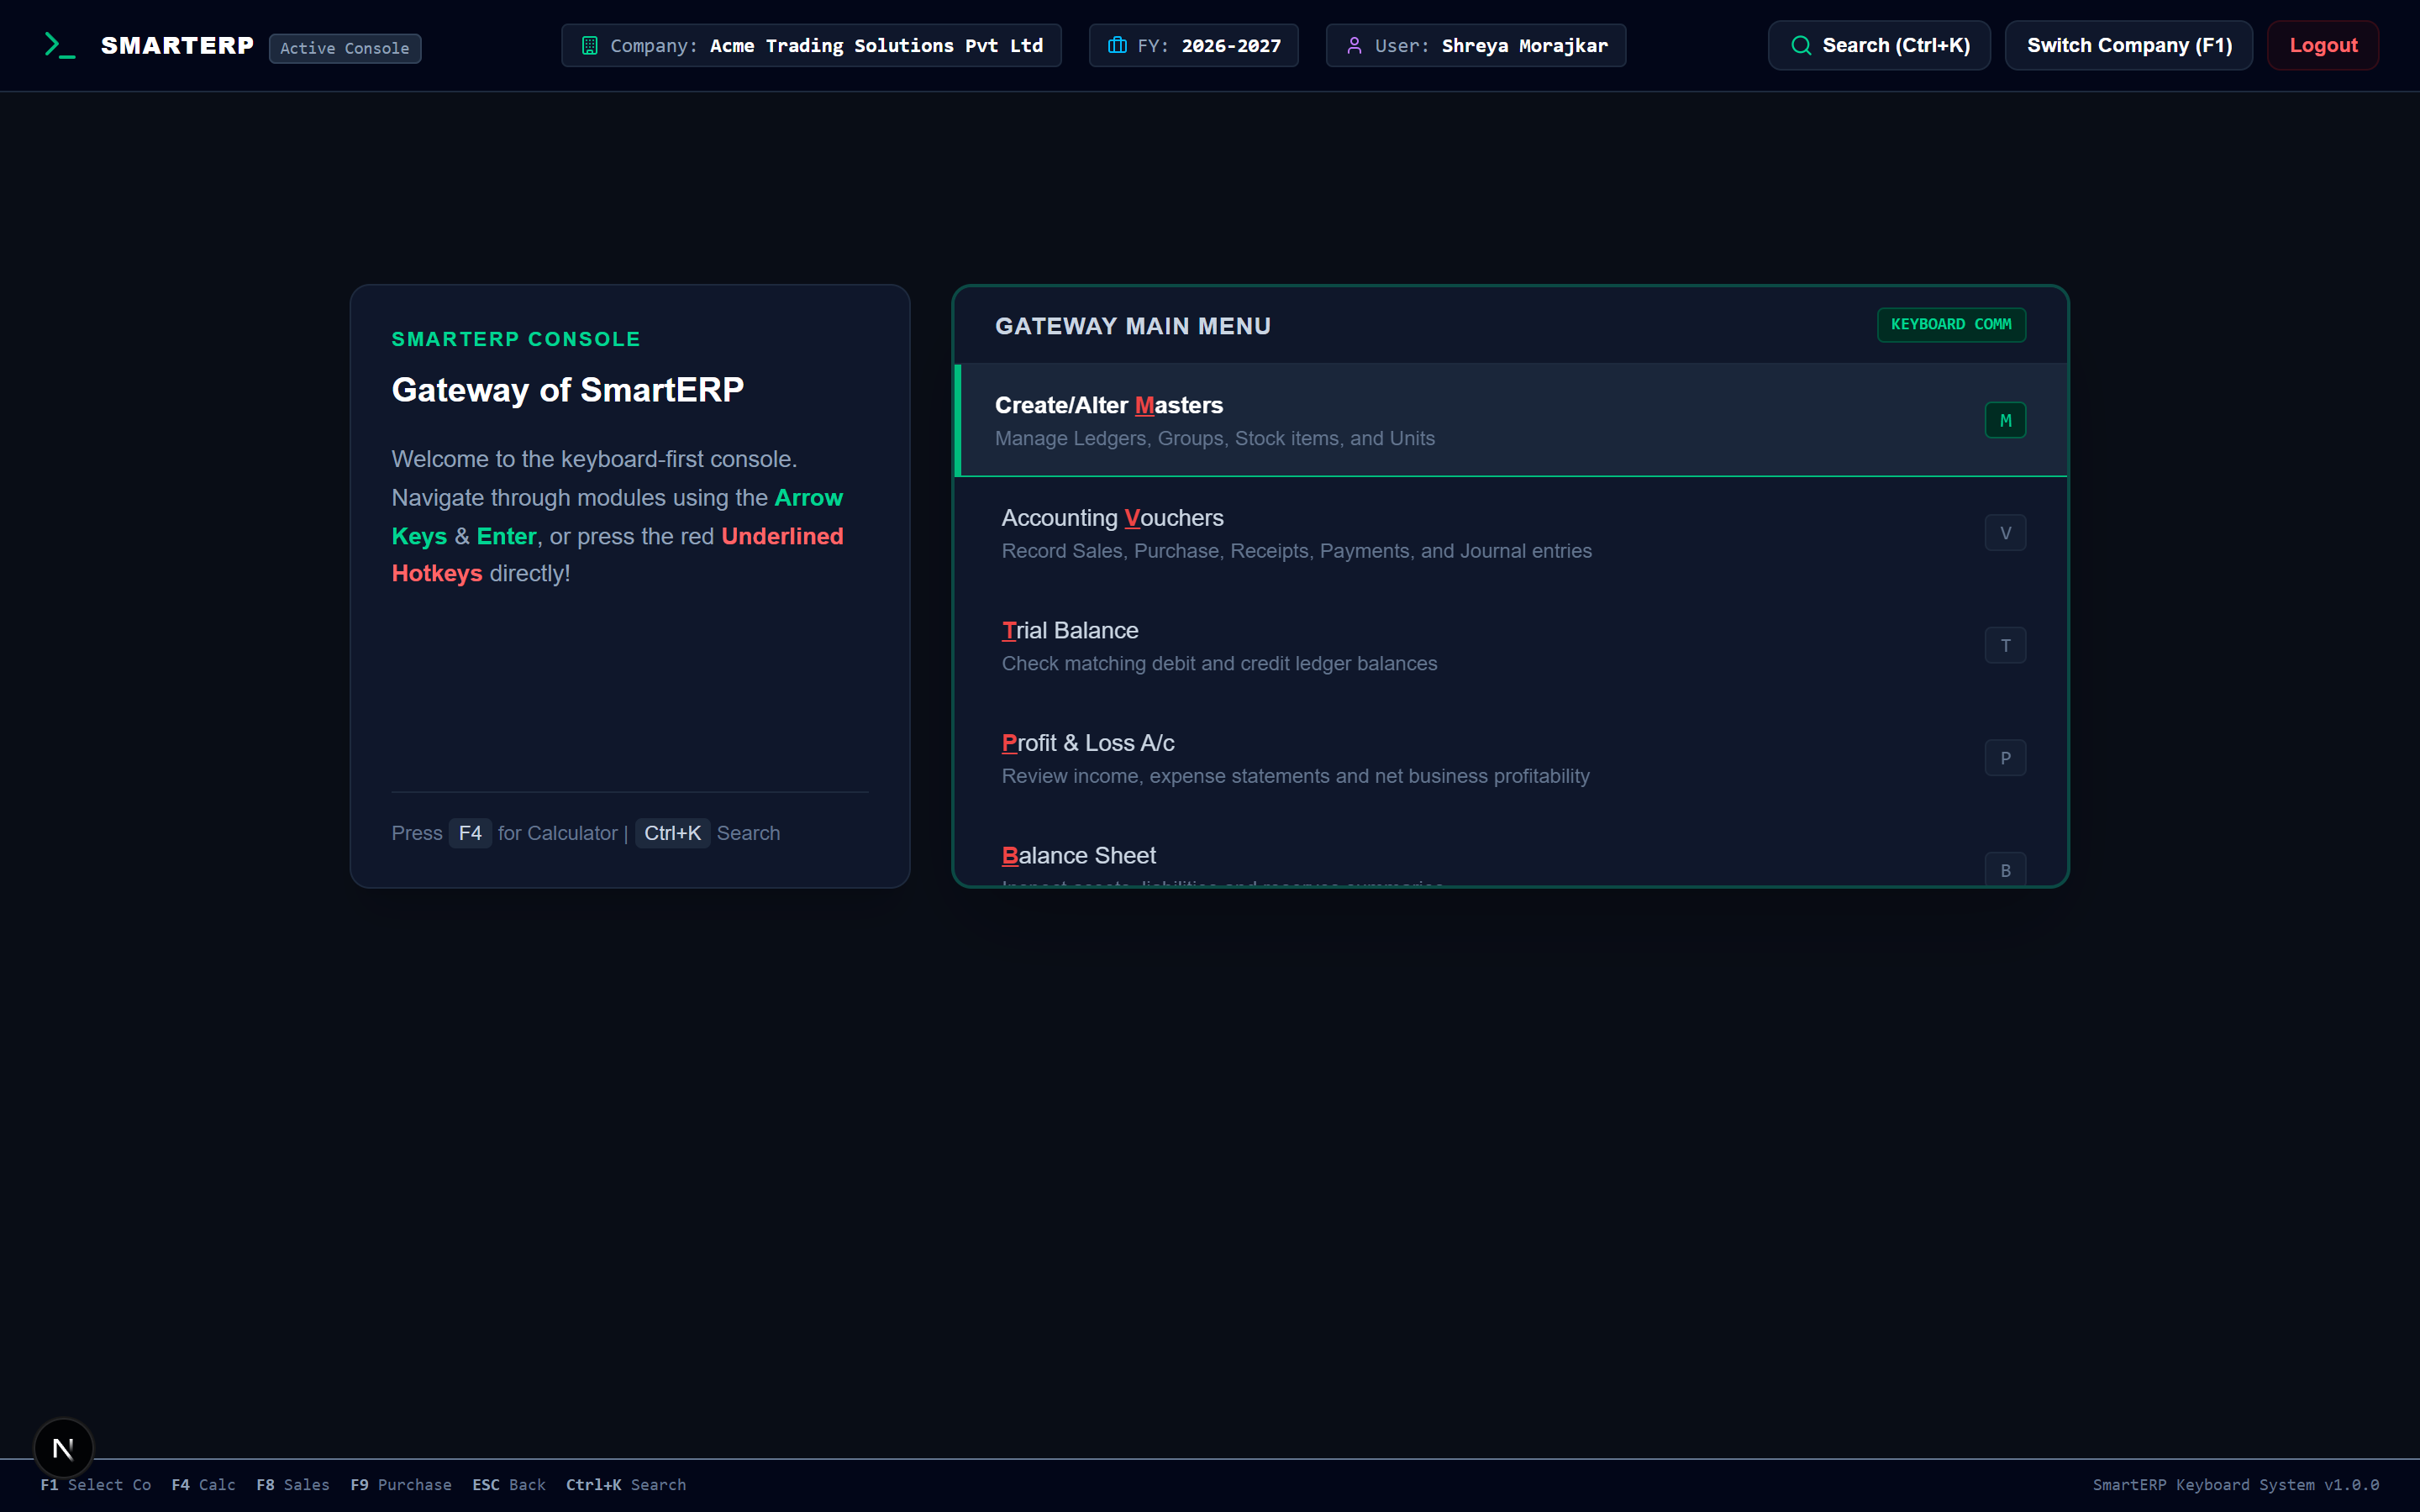
\includegraphics[width=0.85\textwidth]{images/03_gateway_dashboard.png}
  \caption{Gateway Dashboard of SmartERP displaying hotkey-driven navigation}
  \label{fig:architecture}
\end{figure}

The application flow comprises:
\begin{enumerate}
    \item \textbf{Presentation Layer}: Next.js React components rendering reactive ledger grids, voucher allocation tables, and financial statements. Global keyboard events are captured via a dedicated \texttt{useKeyboardShortcuts} React hook.
    \item \textbf{Application \& Business Layer}: Express.js REST API providing modular endpoints for authentication, company management, master creation, voucher processing, tax calculations, and file generation.
    \item \textbf{Database \& ORM Layer}: Prisma ORM mapping type-safe schema definitions into transactional SQL queries, guaranteeing ACID compliance for financial mutations.
\end{enumerate}

\section{Database Modeling and Schema Design}
The relational database schema is structured around double-entry accounting principles and multi-tenant isolation. Table~\ref{tab:schema-summary} summarizes the primary database models.

\begin{table}[htbp]
\centering
\caption{SmartERP Primary Database Entities and Relationships}
\label{tab:schema-summary}
\begin{tabular}{llp{7.5cm}}
\toprule
\textbf{Entity Name} & \textbf{Primary Key} & \textbf{Functional Description} \\
\midrule
\texttt{User} & \texttt{id} (UUID) & System administrator credentials with bcrypt-hashed passwords. \\
\texttt{Company} & \texttt{id} (UUID) & Multi-tenant business workspace with GSTIN and state info. \\
\texttt{Group} & \texttt{id} (UUID) & Chart of Accounts categories (\textit{Assets, Liabilities, Income, Expenses}). \\
\texttt{Ledger} & \texttt{id} (UUID) & Individual party and nominal accounts maintaining current balances. \\
\texttt{StockItem} & \texttt{id} (UUID) & Inventory items with SKU, HSN, rates, GST \%, and stock counts. \\
\texttt{Voucher} & \texttt{id} (UUID) & Transaction header storing type (\textit{SALES, PURCHASE, etc.}) and total. \\
\texttt{VoucherEntry} & \texttt{id} (UUID) & Atomic double-entry lines recording debit and credit amounts. \\
\texttt{GSTRecord} & \texttt{id} (UUID) & Tax audit records recording CGST, SGST, and IGST breakdowns. \\
\bottomrule
\end{tabular}
\end{table}

\section{Core Modules Implementation}

\subsection{Multi-Tenant Company Initialization and Auto-Seeding}
Upon creating a new company, the backend executes an atomic transaction that provisions the company record and seeds the four primary accounting groups along with default system ledgers:
\begin{itemize}
    \item \textbf{Primary Groups}: \textit{Assets (ASSET), Liabilities (LIABILITY), Income (INCOME), Expenses (EXPENSE)}.
    \item \textbf{System Ledgers}: \textit{Cash (Asset), Bank (Asset)}.
\end{itemize}

\subsection{Double-Entry Voucher and Inventory Transaction Engine}
When a user records a voucher (e.g., Sales or Purchase), the backend executes a Prisma transaction (\texttt{tx.\$transaction}) ensuring all balance and stock updates occur atomically:
\begin{enumerate}
    \item Creates the parent \texttt{Voucher} record with unique sequence numbering.
    \item Writes individual \texttt{VoucherEntry} debit and credit records.
    \item Mutates the current balance of affected ledgers:
    \begin{equation}
      \text{Balance}_{\text{new}} = 
      \begin{cases}
        \text{Balance}_{\text{old}} + \text{Debit} - \text{Credit}, & \text{for Asset / Expense Ledgers} \\
        \text{Balance}_{\text{old}} + \text{Credit} - \text{Debit}, & \text{for Liability / Income Ledgers}
      \end{cases}
    \end{equation}
    \item Adjusts inventory quantities (\texttt{currentQty}) in \texttt{StockItem} based on transaction direction ($+\Delta q$ for Purchase, $-\Delta q$ for Sales).
    \item Computes and records applicable GST splits in \texttt{GSTRecord}.
\end{enumerate}

\subsection{State-Aware GST Computation Algorithm}
Algorithm~\ref{alg:gst} formalizes the automated tax determination logic implemented in the billing pipeline.

\begin{algorithm}[htbp]
\caption{State-Aware GST Tax Allocation Engine}
\label{alg:gst}
\begin{algorithmic}[1]
\Require Company State $S_c$, Counterparty State $S_p$, Taxable Amount $A$, GST Rate $R$
\Ensure Total Tax $T$, Tax Breakdown $(\text{CGST}, \text{SGST}, \text{IGST})$
\State $T \gets A \times \left(\frac{R}{100}\right)$
\If{$\text{Normalize}(S_c) = \text{Normalize}(S_p)$} \Comment{Intra-State Transaction}
    \State $\text{CGST} \gets \frac{T}{2}$
    \State $\text{SGST} \gets \frac{T}{2}$
    \State $\text{IGST} \gets 0$
\Else \Comment{Inter-State Transaction}
    \State $\text{CGST} \gets 0$
    \State $\text{SGST} \gets 0$
    \State $\text{IGST} \gets T$
\EndIf
\State \Return $T, (\text{CGST}, \text{SGST}, \text{IGST})$
\end{algorithmic}
\end{algorithm}

\subsection{Keyboard Navigation and Productivity Engine}
To provide high-speed data entry, a custom React hook intercepts browser keyboard events:
\begin{itemize}
    \item \textbf{Function Keys}: $F1$ (Switch Company), $F4$ (Floating Calculator Overlay), $F8$ (Sales Voucher), $F9$ (Purchase Voucher), $F5$--$F7$ (Payment, Receipt, Journal).
    \item \textbf{Spotlight Search ($Ctrl+K$)}: Opens a fuzzy-search palette to jump instantly to any ledger, item, or report.
    \item \textbf{Underlined Hotkeys}: Pressing highlighted hotkey letters directly on menu cards ($M$ for Masters, $V$ for Vouchers, $T$ for Trial Balance) triggers immediate routing.
\end{itemize}

\begin{figure}[htbp]
  \centering
  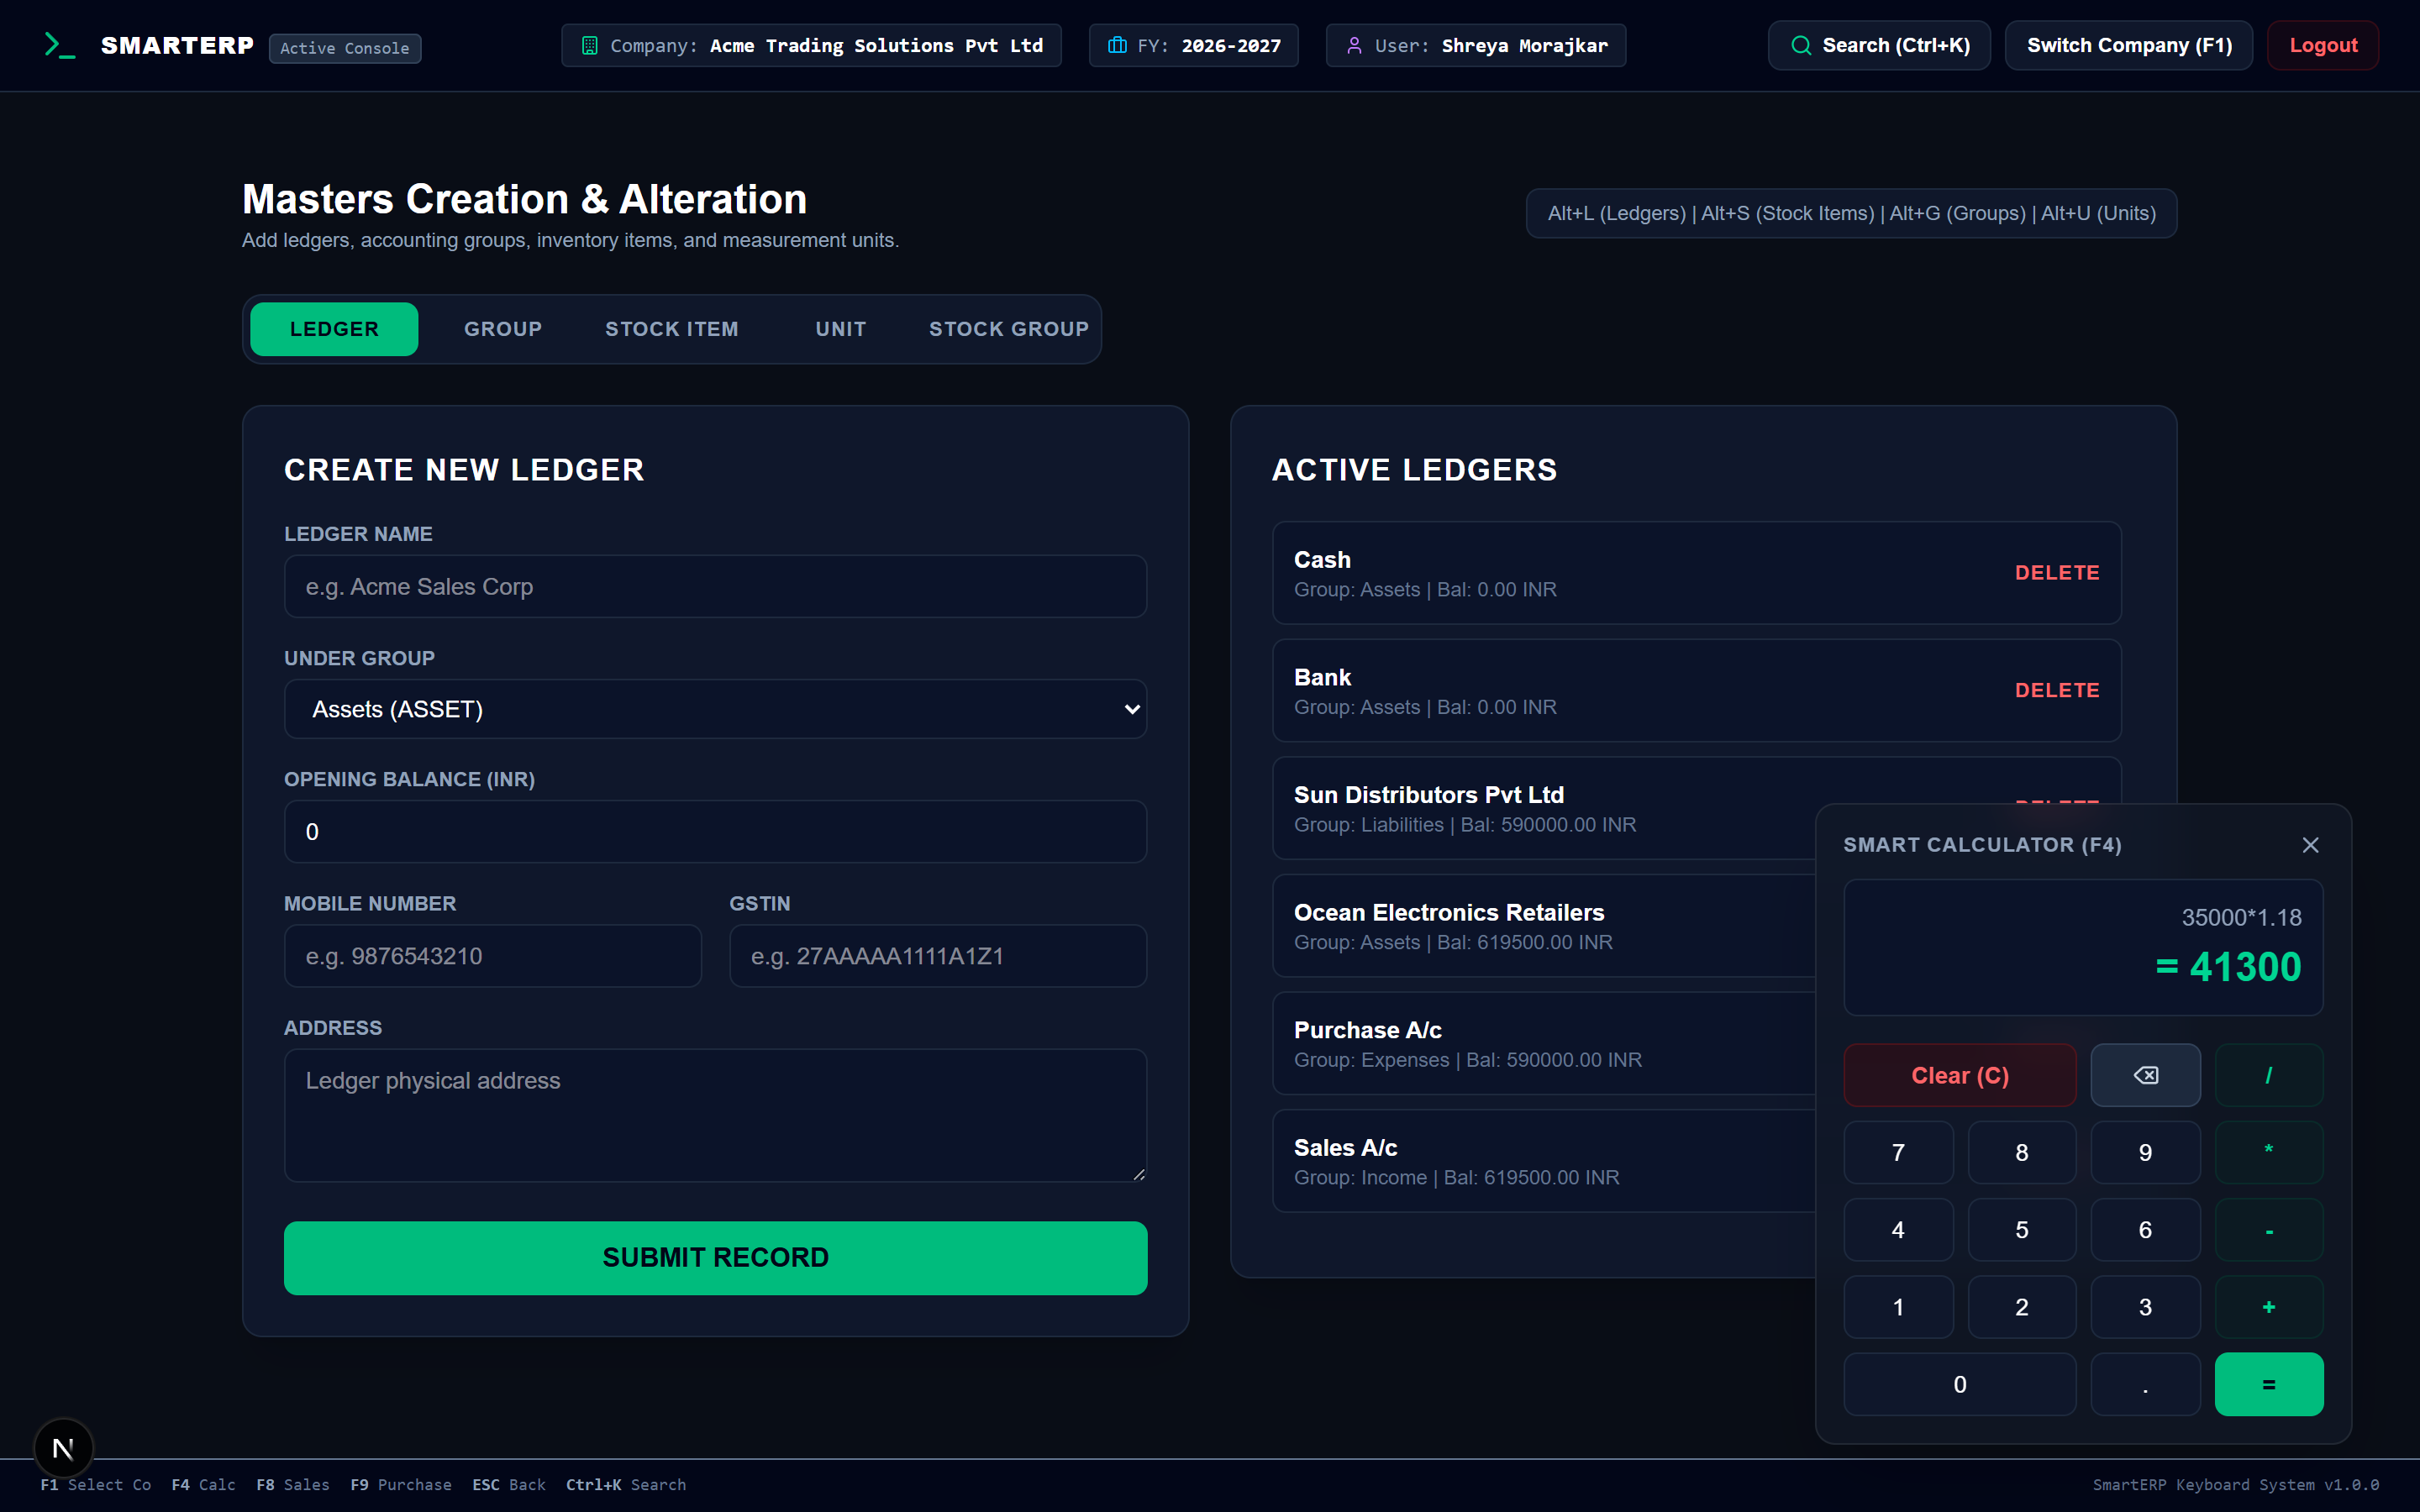
\includegraphics[width=0.85\textwidth]{images/04_calculator_overlay.png}
  \caption{Context-preserving floating calculator overlay ($F4$) during ledger management}
  \label{fig:calculator}
\end{figure}

\subsection{Real-Time Financial Reporting and Verification}
Financial statements are dynamically generated from ledger entries:
\begin{itemize}
    \item \textbf{Trial Balance}: Computes cumulative debits ($\sum Dr$) and credits ($\sum Cr$) verifying the fundamental accounting equation:
    \begin{equation}
      \sum_{i=1}^{n} \text{Debit}_i = \sum_{j=1}^{m} \text{Credit}_j
    \end{equation}
    \item \textbf{Profit \& Loss Account}: Computes Gross and Net Income derived from total Income ledger credits minus Expense ledger debits.
    \item \textbf{Balance Sheet}: Verifies that $\text{Total Assets} = \text{Total Liabilities} + \text{Equity/Reserves}$.
    \item \textbf{Stock Valuation}: Evaluates warehouse asset value:
    \begin{equation}
      \text{Valuation} = \sum_{k=1}^{p} (\text{CurrentQty}_k \times \text{PurchaseRate}_k)
    \end{equation}
\end{itemize}

\section{Automated Integration Testing and Results}
An automated test harness (\texttt{test\_features.js}) was developed to validate all accounting operations programmatically. Table~\ref{tab:test-results} summarizes the validation results.

\begin{table}[htbp]
\centering
\caption{Automated Integration Test Verification Results}
\label{tab:test-results}
\begin{tabular}{lp{6.0cm}cc}
\toprule
\textbf{Test Module} & \textbf{Verification Target} & \textbf{Expected Output} & \textbf{Status} \\
\midrule
User Authentication & Admin registration \& JWT issuance & Token Generated & \textbf{PASS} \\
Company Seeding & Auto-creation of 4 groups \& 2 ledgers & Groups/Ledgers Verified & \textbf{PASS} \\
Purchase Voucher & Inward 20 TVs @ \text{INR} 25k + 18\% GST & Stock: 120, Liab: \text{INR} 590k & \textbf{PASS} \\
Sales Voucher & Outward 15 TVs @ \text{INR} 35k + 18\% GST & Stock: 105, Asset: \text{INR} 619.5k & \textbf{PASS} \\
Trial Balance & Mathematical balance of Debits vs Credits & $\sum Dr = \sum Cr$ & \textbf{PASS} \\
GST Register & Intra-state CGST + SGST tax allocation & CGST: 50\%, SGST: 50\% & \textbf{PASS} \\
PDF Invoice Export & Vector PDF generation with HSN \& GST & HTTP 200 (application/pdf) & \textbf{PASS} \\
Excel Export & Spreadsheet workbook generation & HTTP 200 (.xlsx stream) & \textbf{PASS} \\
\bottomrule
\end{tabular}
\end{table}

\chapter{Conclusion and Future Scope}

\section{Conclusion}
The internship at \textbf{Labmentix} provided an invaluable opportunity to design, engineer, and deploy \textbf{SmartERP}---a comprehensive, full-stack enterprise resource planning and billing platform. By bridging the gap between the keyboard-driven efficiency of legacy desktop systems like Tally and the collaborative power of modern cloud technologies, the project demonstrated that web-based accounting can achieve sub-second data-entry throughput with zero user friction.

Throughout the project lifecycle, key technical milestones were accomplished:
\begin{enumerate}
    \item Developed a robust, decoupled full-stack architecture using Next.js 16, React 19, Node.js, Express, and Prisma ORM.
    \item Implemented an event-driven keyboard shortcuts engine ($F1$--$F9$, underlined hotkeys, $Ctrl+K$ spotlight search, $F4$ calculator overlay) that allows 100\% mouse-free accounting workflows.
    \item Enforced mathematical consistency in double-entry bookkeeping using atomic database transactions.
    \item Integrated automated state-aware Indian GST computation (CGST, SGST, IGST) with real-time financial reporting (Trial Balance, P\&L, Balance Sheet, Stock Summary) and instant PDF/Excel exports.
    \item Verified system reliability through an automated end-to-end integration test harness with a 100\% success rate.
\end{enumerate}

\section{Key Learnings}
The internship significantly enhanced practical engineering competence in several core domains:
\begin{itemize}
    \item \textbf{Full-Stack System Design}: Building production-ready RESTful APIs and optimizing React rendering cycles in Next.js App Router.
    \item \textbf{Transactional Integrity in ORMs}: Utilizing Prisma \texttt{\$transaction} blocks to manage multi-table financial operations without race conditions.
    \item \textbf{Domain Knowledge in Accounting \& Taxation}: Understanding the double-entry accounting equation, Chart of Accounts hierarchy, inventory valuation models, and statutory GST compliances.
    \item \textbf{Test-Driven Verification}: Writing automated integration tests to simulate realistic multi-voucher transaction flows.
\end{itemize}

\section{Future Scope}
While SmartERP currently delivers a complete billing and accounting workflow, future development roadmaps include:
\begin{itemize}
    \item \textbf{Statutory e-Way Bill \& e-Invoice API Integration}: Direct integration with the Government of India GST Portal (NIC APIs) for automatic IRN (Invoice Reference Number) and e-Way bill generation.
    \item \textbf{Barcode \& POS Scanner Hardware Support}: Native USB/Bluetooth barcode scanner integration for high-speed retail checkout scanning.
    \item \textbf{Multi-Currency Accounting}: Real-time foreign exchange rate conversion for international trade and cross-border invoicing.
    \item \textbf{Role-Based Access Control (RBAC)}: Granular permission levels for Accountants, Auditors, Inventory Clerks, and Billing Executives.
\end{itemize}

\appendix

\begingroup
\titleformat{\chapter}[display]
  {\bfseries\centering}
  {}
  {6pt}
  {\MakeUppercase}

\refstepcounter{chapter}
\chapter*{Appendices}
\addcontentsline{toc}{chapter}{Appendices}

\section{Offer Letter}
\noindent\begin{center}
  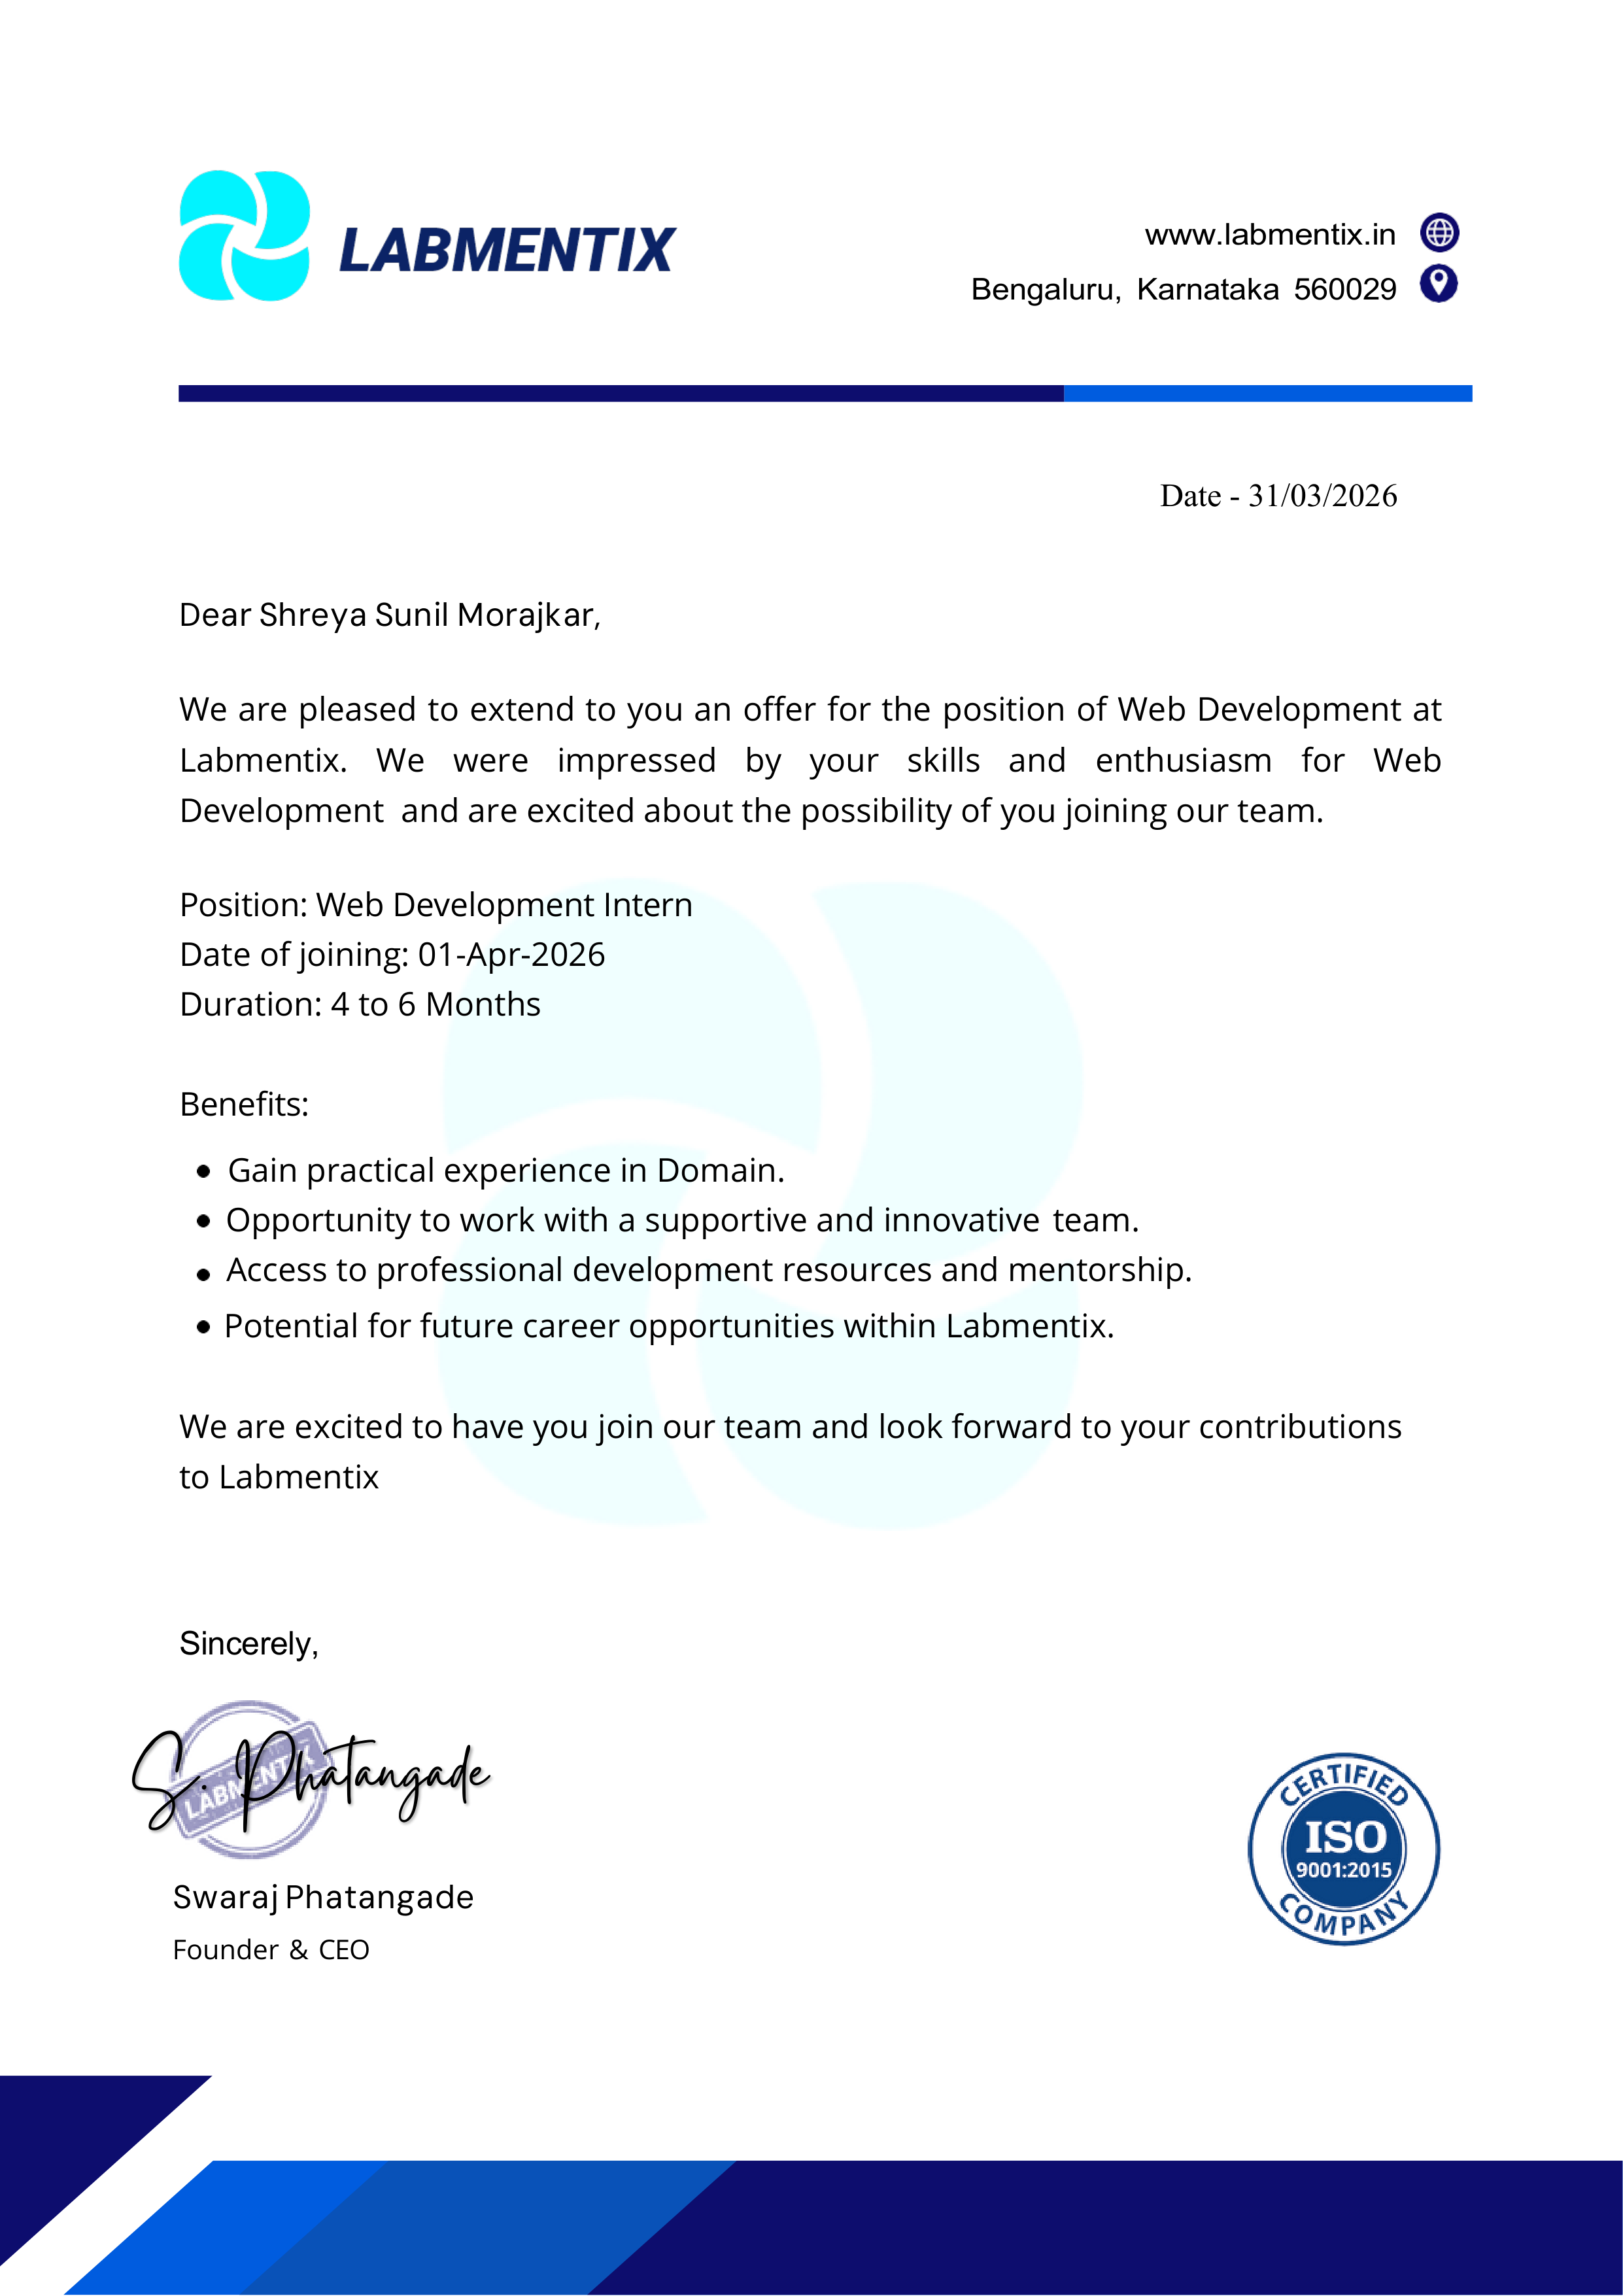
\includegraphics[width=0.92\textwidth]{images/offer_letter.png}
\end{center}
\clearpage

\section{Completion Certificate}
\noindent\begin{center}
  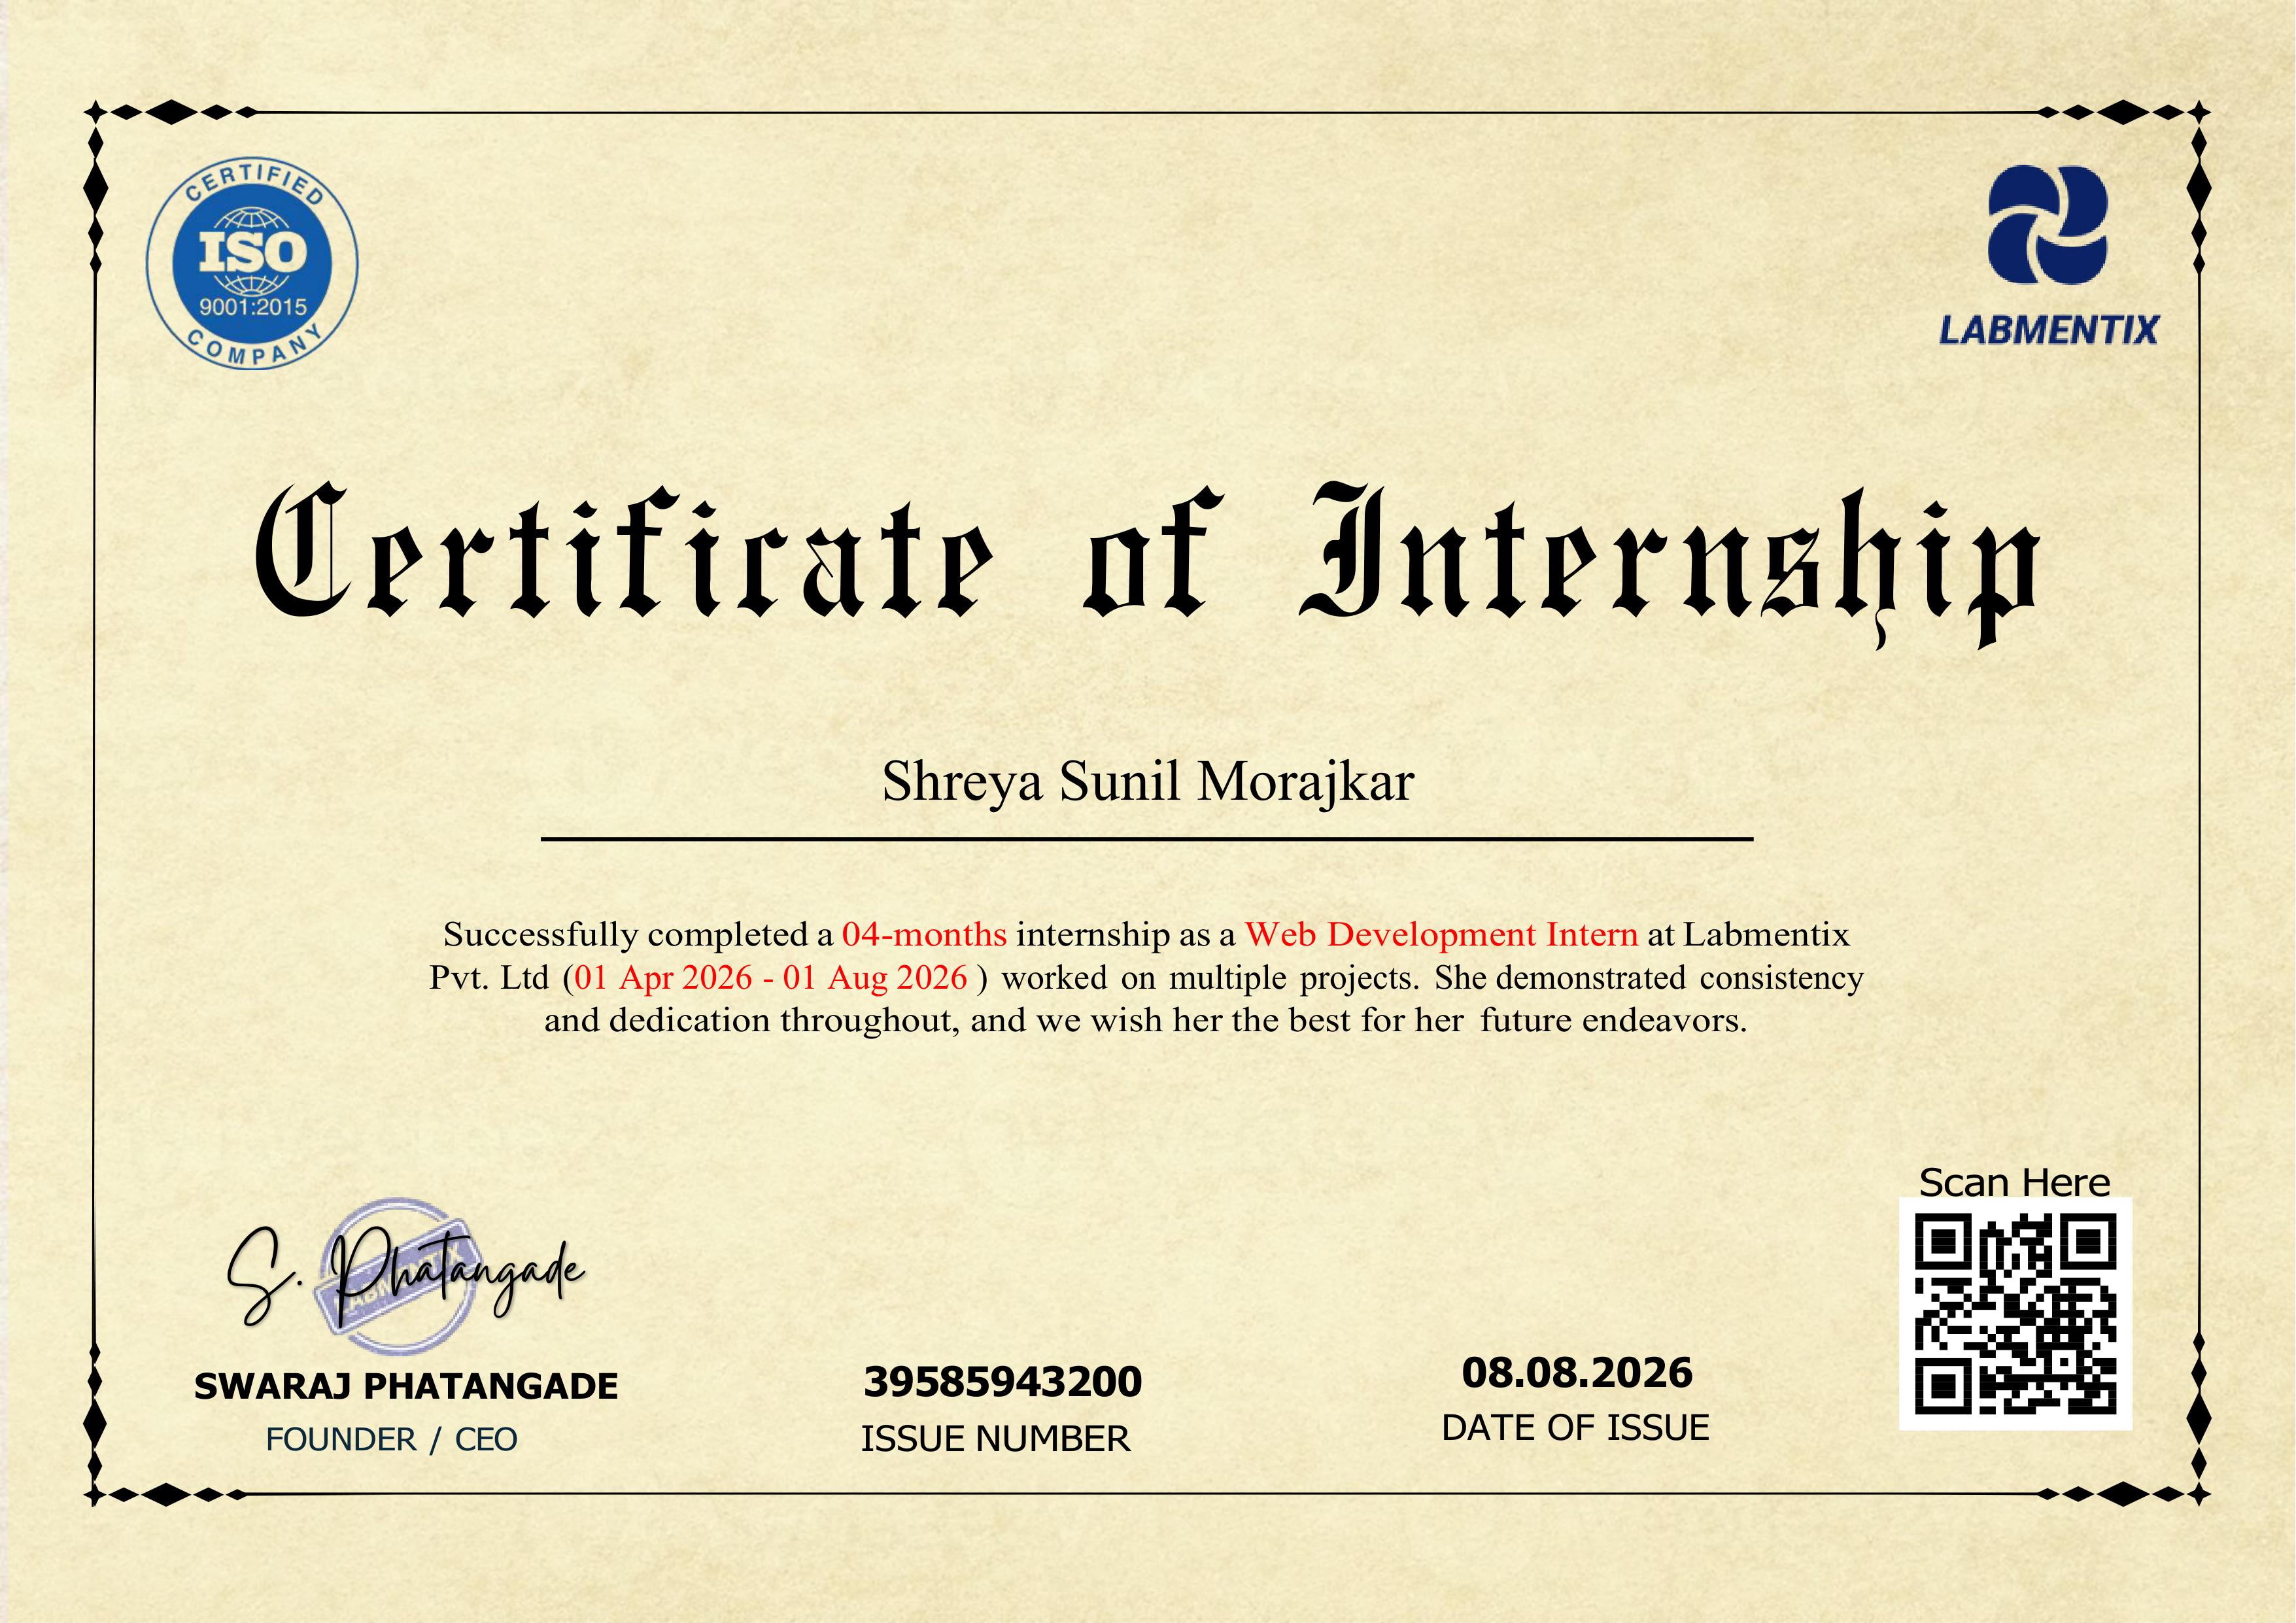
\includegraphics[width=0.92\textwidth]{images/completion_certificate.png}
\end{center}
\clearpage

\section{SmartERP Application Screenshots}

\subsection{Sales Invoice Voucher Entry ($F8$)}
\noindent\begin{center}
  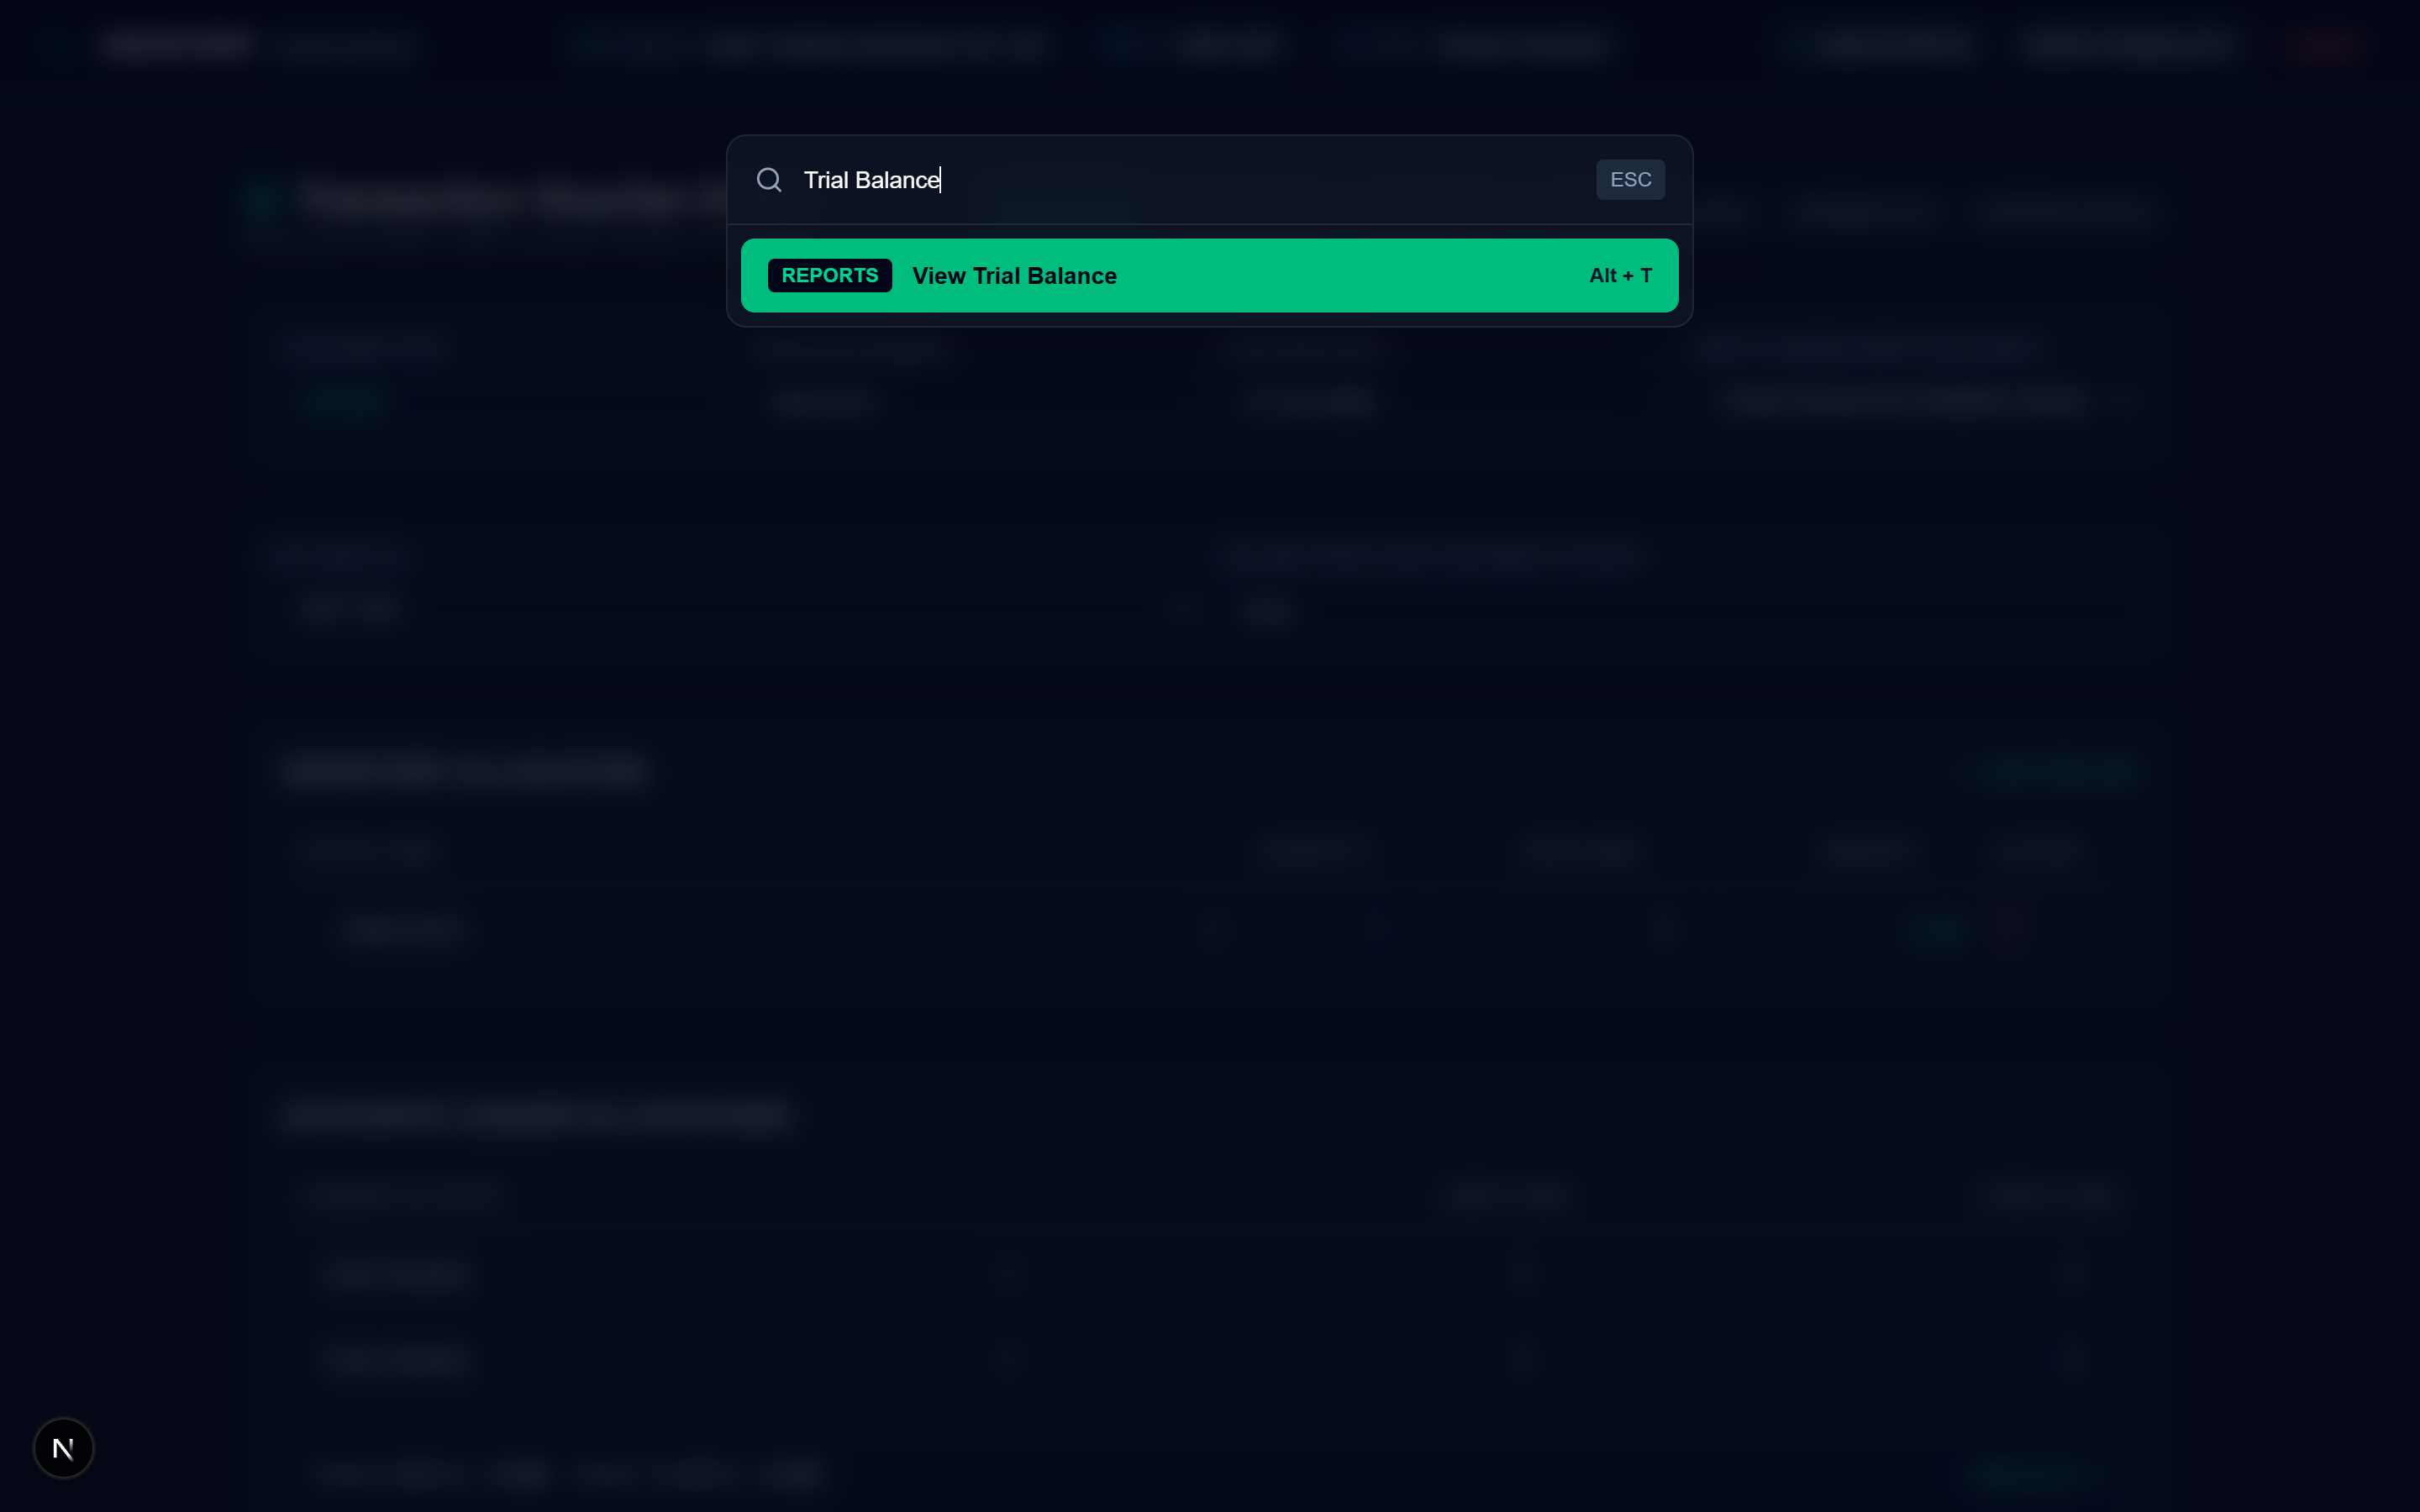
\includegraphics[width=0.95\textwidth]{images/08_voucher_entry_sales.png}
\end{center}
\clearpage

\subsection{Real-Time Trial Balance Statement ($Alt + T$)}
\noindent\begin{center}
  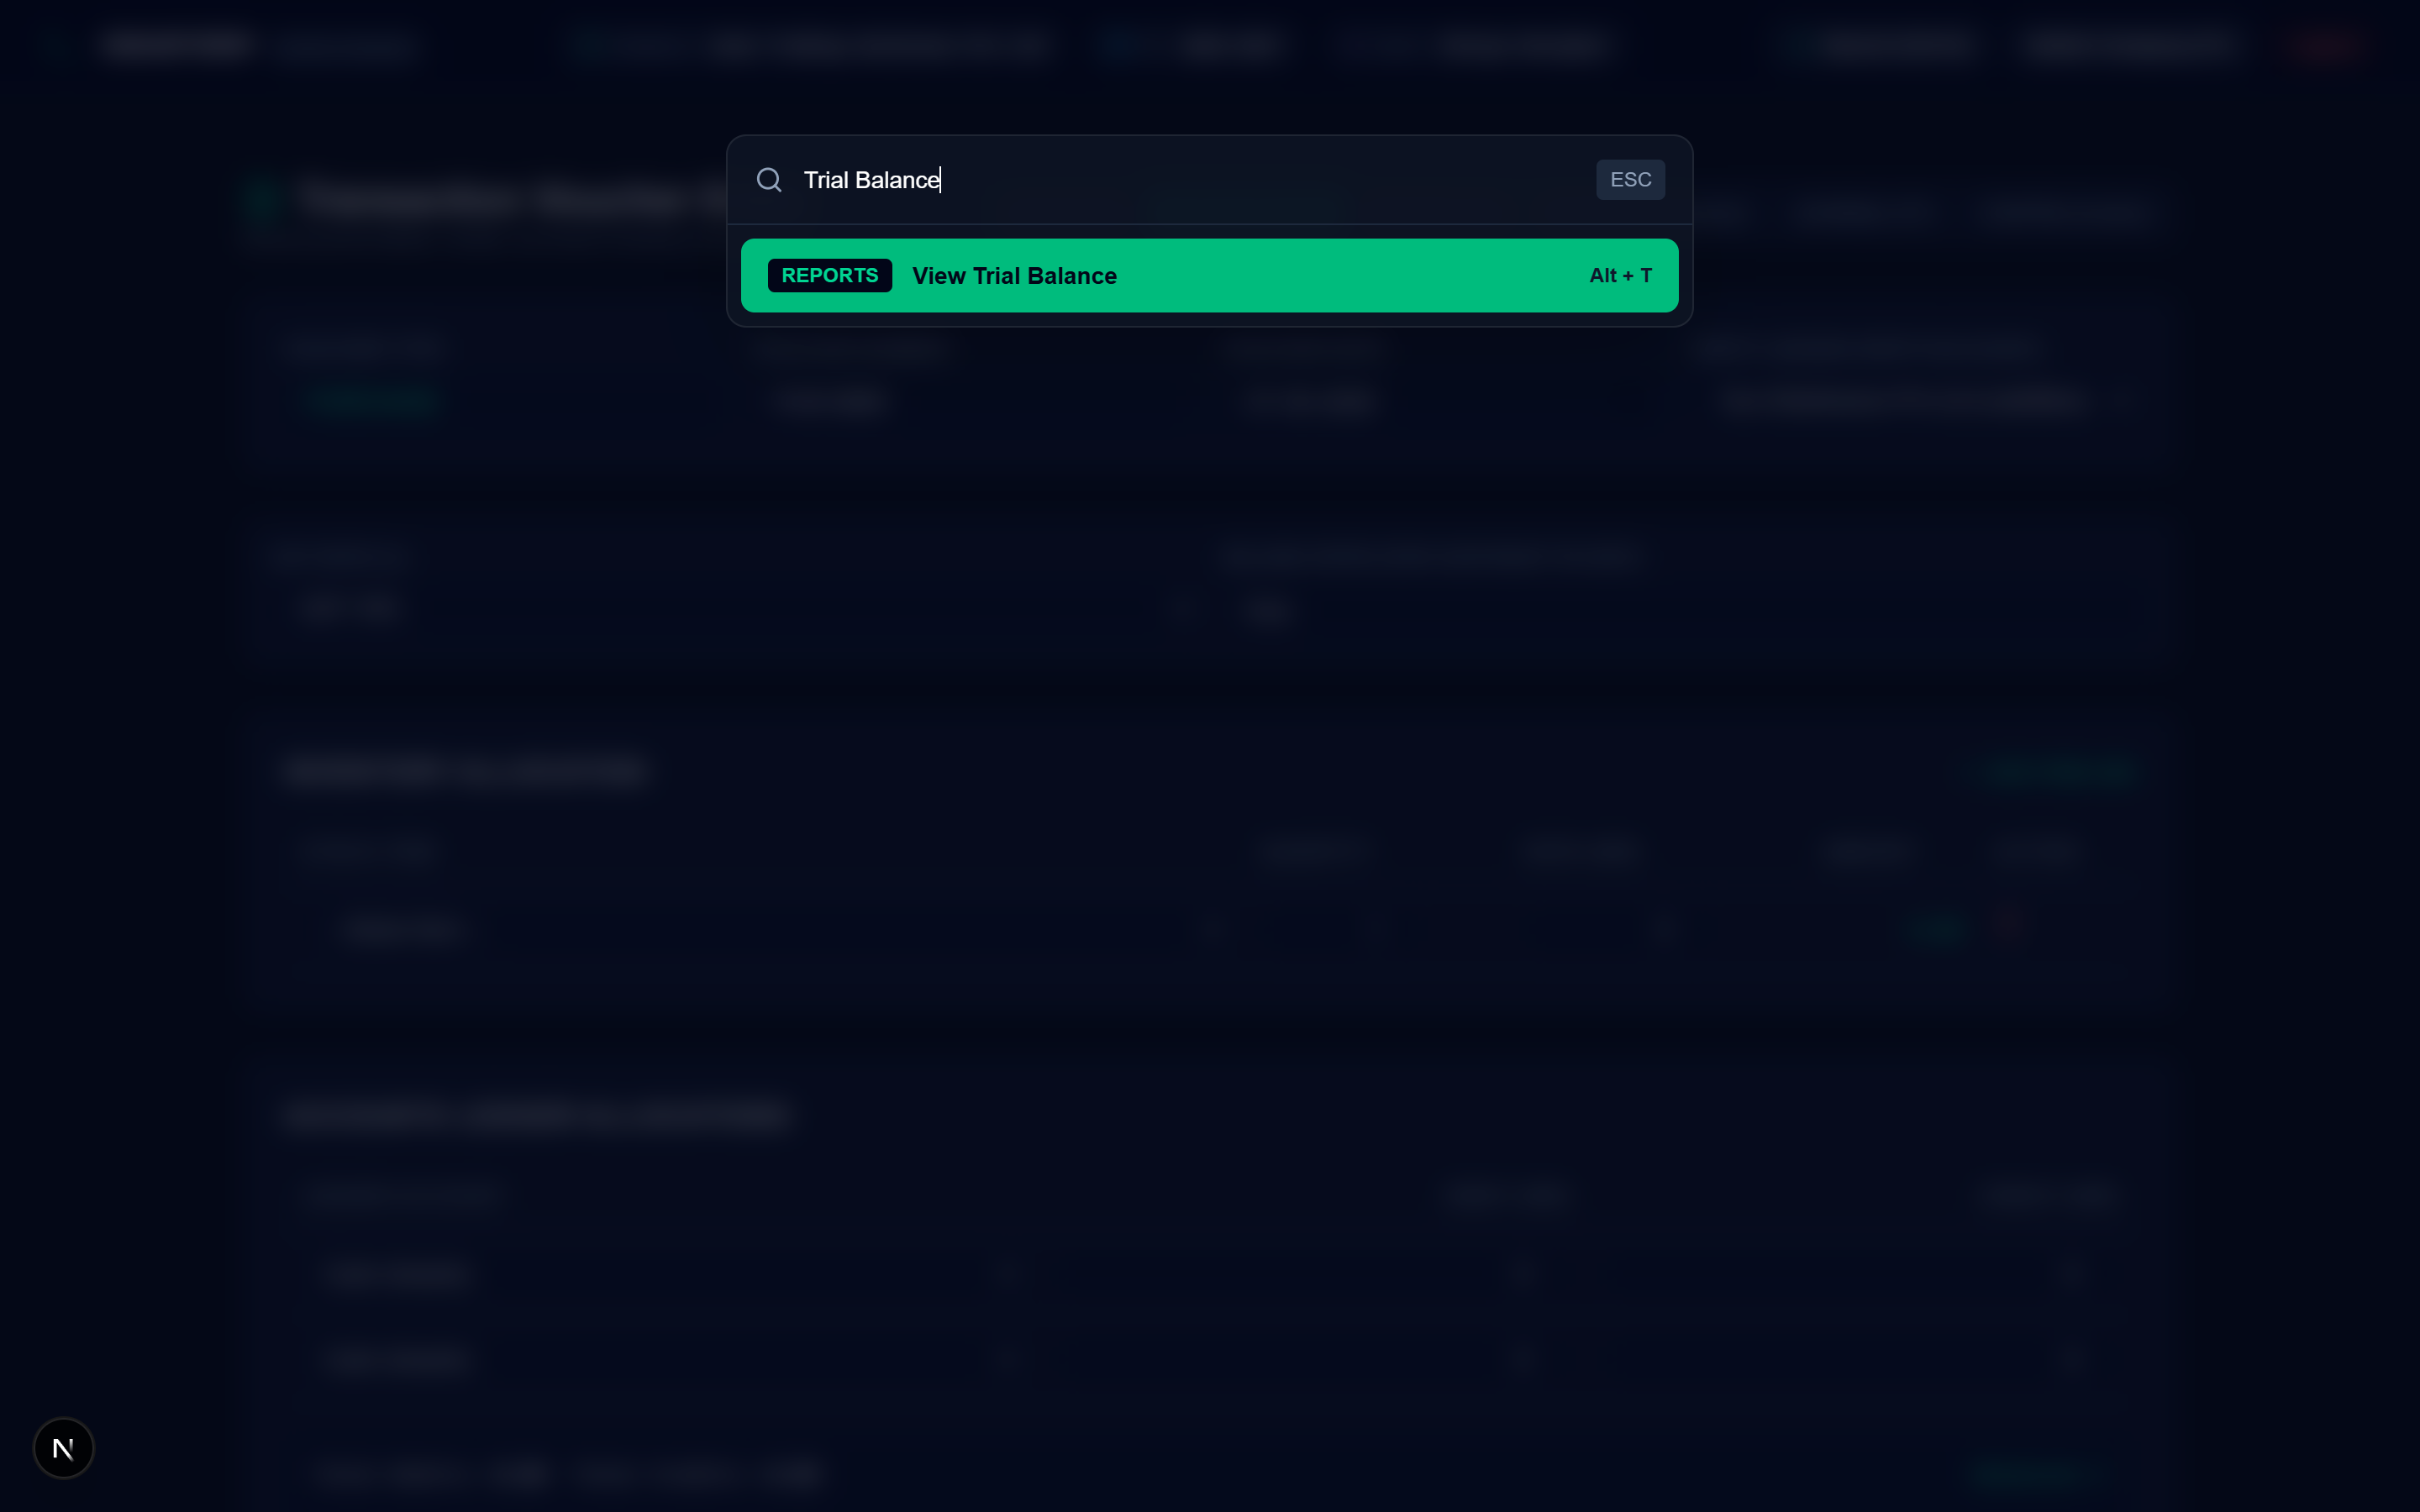
\includegraphics[width=0.95\textwidth]{images/10_trial_balance_report.png}
\end{center}
\clearpage

\subsection{GST Tax Register and GSTR Summary ($Alt + X$)}
\noindent\begin{center}
  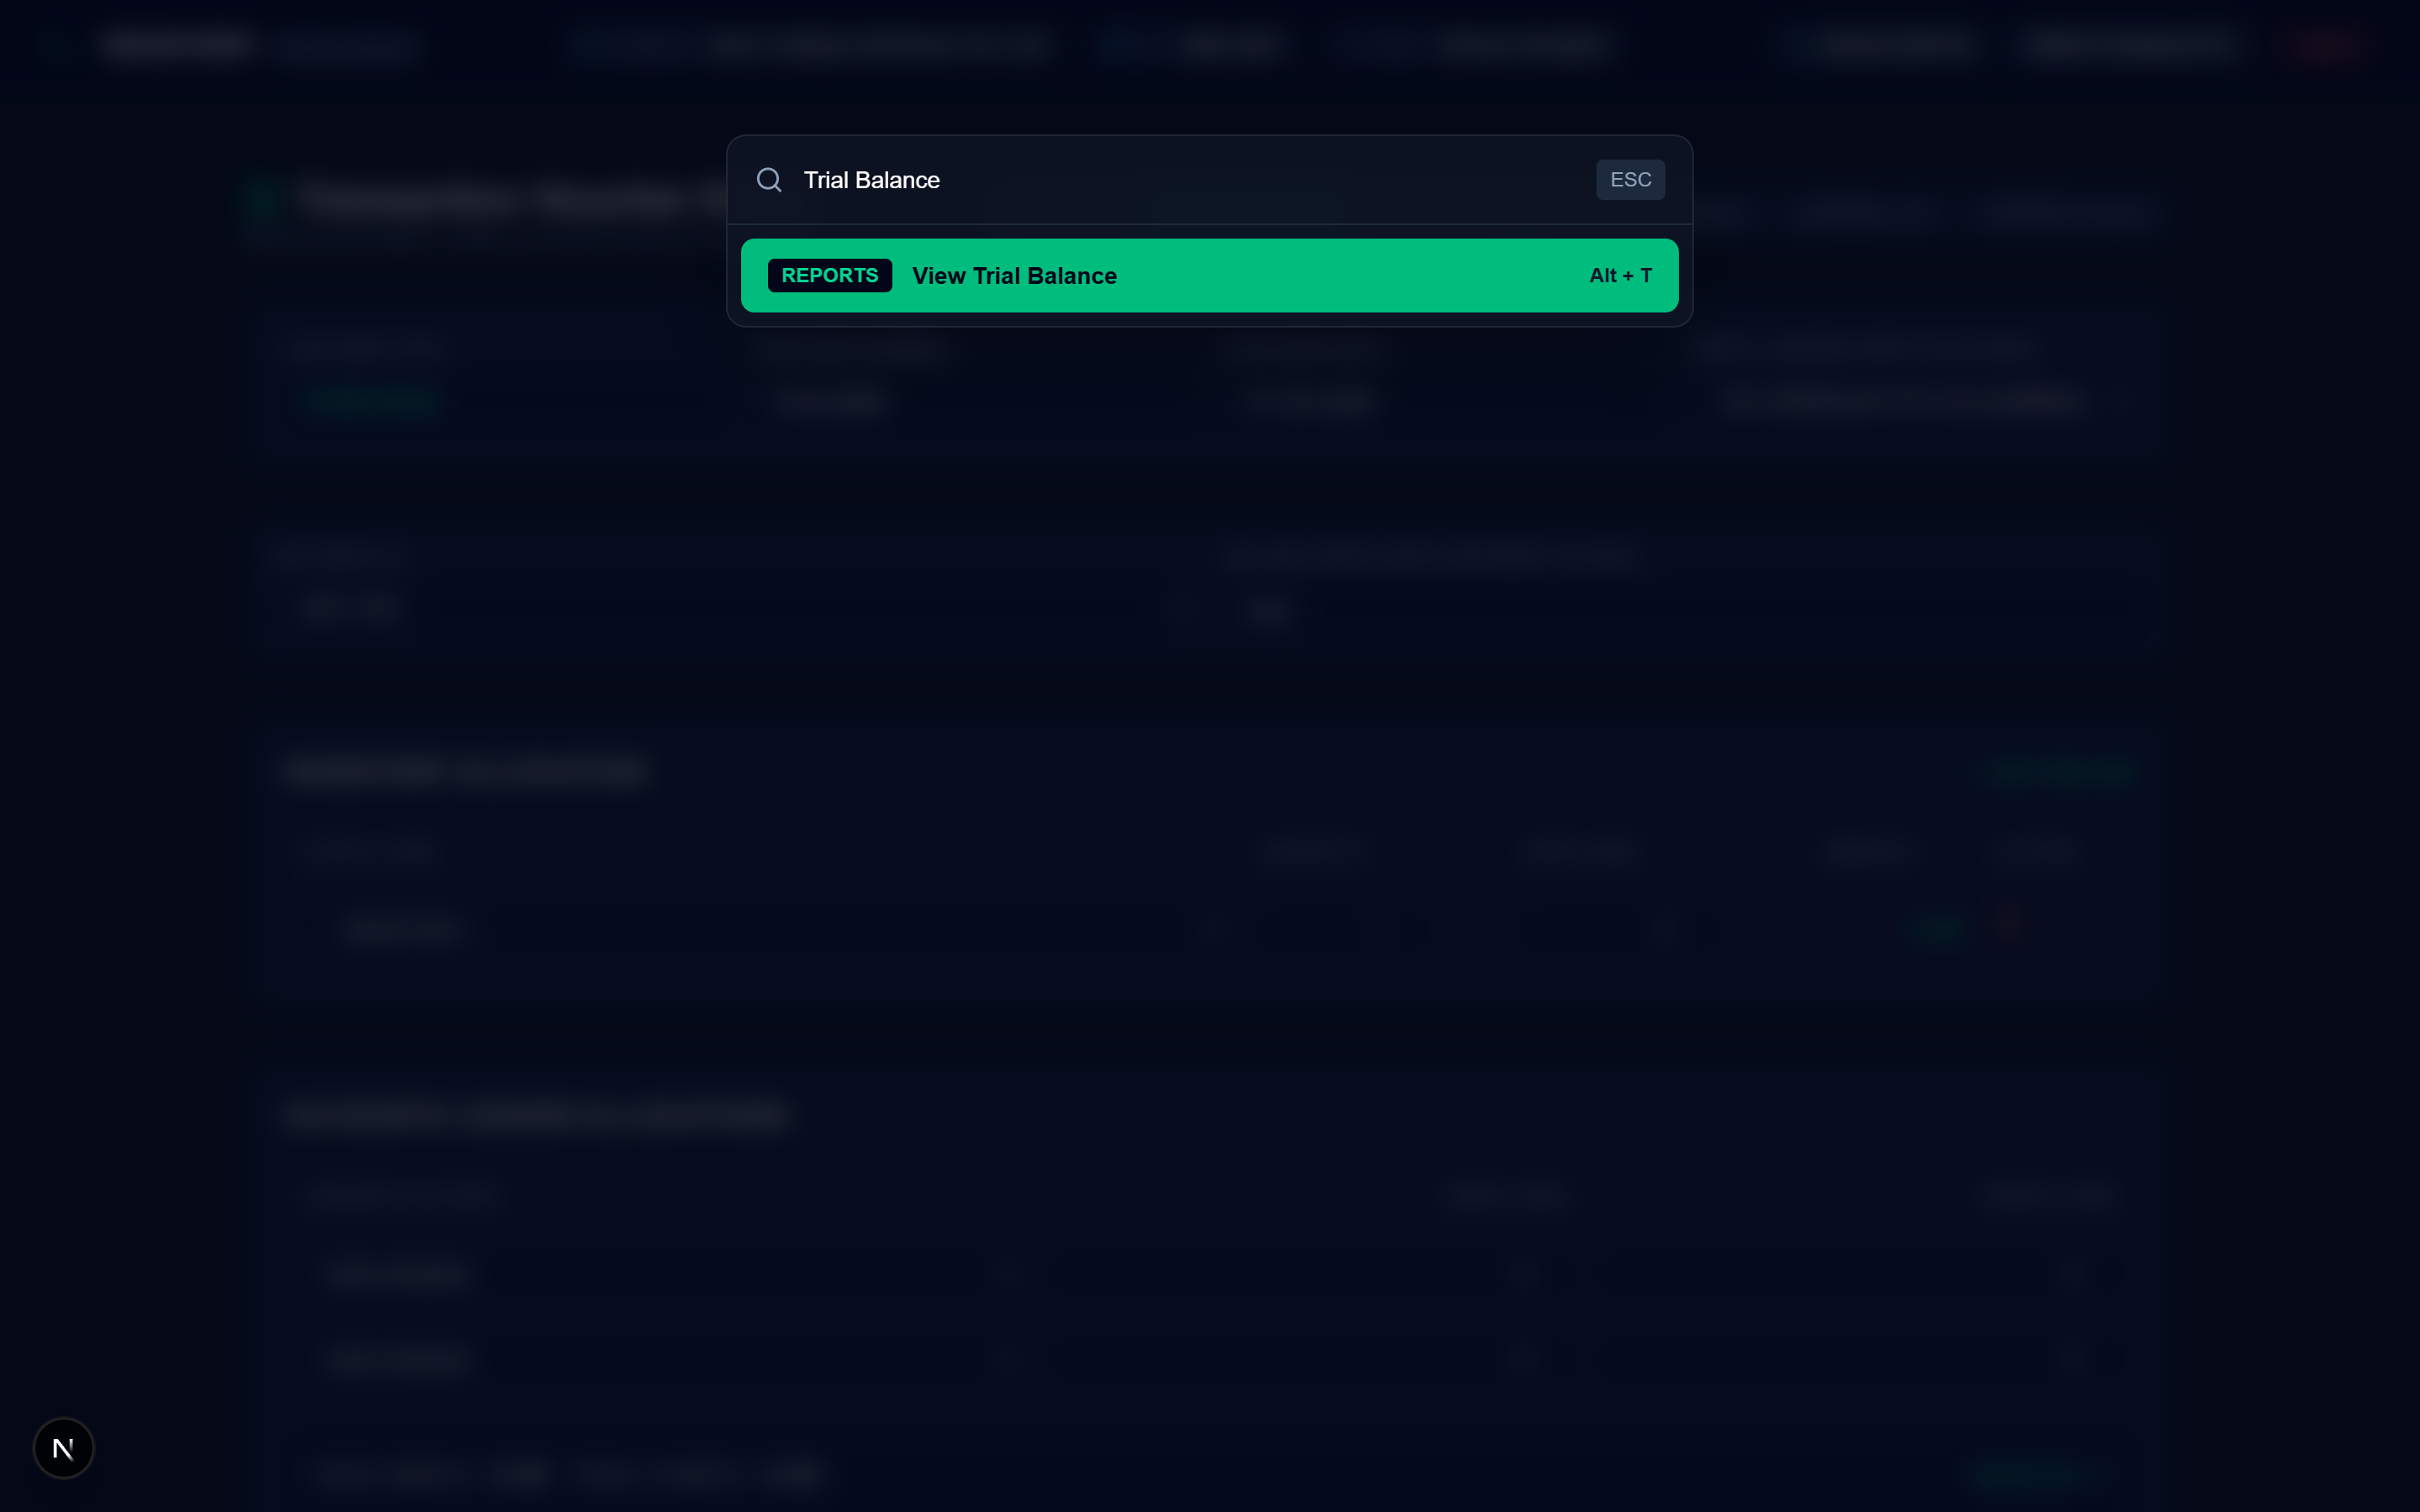
\includegraphics[width=0.95\textwidth]{images/14_gst_register_report.png}
\end{center}
\clearpage

\endgroup


% ===== References =====
\cleardoublepage
\addcontentsline{toc}{chapter}{\bibname}
\nocite{sommerville2016,nextjs2024,prisma2024,tallyerp2023,doubleentry2022}
\bibliographystyle{IEEEtran}
\bibliography{references}

\end{document}
